% Based on the ACM SIG Proceedings sample. The KDD Research CFP specifies
% sigconf,anonymous,review. Overleaf root document: main.tex.
% The original vector overview is PDF 1.7.
\ifdefined\pdfminorversion\pdfminorversion=7\relax\fi
\documentclass[sigconf,anonymous,review]{acmart}
\setcopyright{none}
\acmDOI{}
\acmISBN{}
\acmConference[KDD 2027 Research Track]{KDD 2027 Research Track}{August 2027}{San Jose, CA, USA}
\acmBooktitle{Manuscript prepared for the KDD 2027 Research Track}
\acmYear{2027}
\usepackage{amsmath}
\usepackage{array}

\begin{document}
\title[Same Evidence, Different Estimates]{Same Evidence, Different Estimates: How Modeling Choices Shape Analyses of Agent-Generated Biomedical Data}
\author{Anonymous Author(s)}

\begin{abstract}
Two virtual datasets can reproduce a paper's published biomarker summaries and still give different answers to a screening question. We study which answers depend on how a scientific agent builds the data. The agent reads an article, identifies the quantities it reports, and writes a program that generates individual records. We isolate the choice of which measurements belong to the same person by fixing every value in each column. In a cholesterol study, two assignments returned by one agent reproduce the published mean individual cholesterol ratio and give the same mean non-HDL cholesterol, yet 9.80\% and 26.17\% of virtual adults cross the same screening threshold. Across twelve matched starts per article, asking explicitly for an alternative that changes the analysis produced a material shift in eleven lipid cases, against zero under an ordinary request for another defensible model. The corresponding counts were eleven versus six for lung function and twelve versus twelve for iron status. We then apply the same analyses to virtual and measured records. An agent's handgrip model predicted a mean absolute between-hand difference of 3.81~kg, compared with 3.30 and 3.78~kg in two independent samples. In a Nigerian iron study, six agents and a statistical generator selected similar dependence models and all overestimated the measured association. These comparisons separate the conclusions supplied by an article from those that depend on the agent's modeling decisions.
\end{abstract}

\ccsdesc[500]{Computing methodologies~Modeling and simulation}
\ccsdesc[300]{Applied computing~Life and medical sciences}
\keywords{scientific agents, synthetic biomedical data, dependence, scientific analysis}

\begin{teaserfigure}
\centering
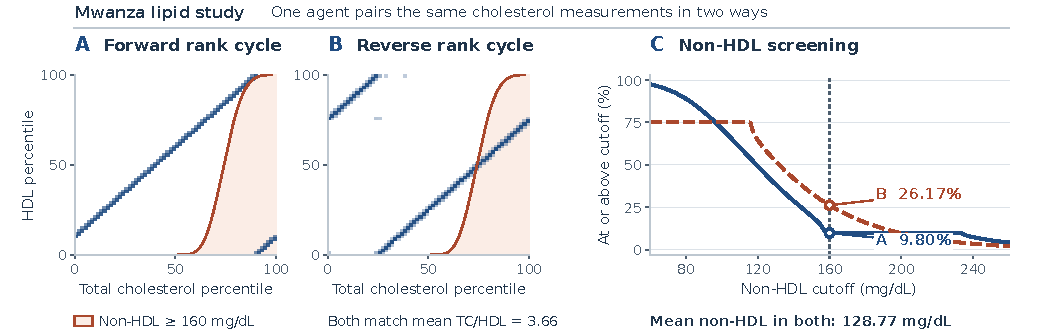
\includegraphics[width=.96\textwidth]{figures/lipid-pairing-overview.pdf}
\caption{How many adults have non-HDL cholesterol of at least 160~mg/dL? An agent paired the same total (TC) and HDL cholesterol values in two ways. In A and B, blue cells show occupied percentile pairs and shading marks the screening region. C shows the fraction above each cutoff. Both assignments give mean non-HDL of 128.77~mg/dL and reproduce the source's mean individual TC/HDL ratio of 3.66. At 160~mg/dL the fractions differ by 16.37 percentage points. This was the smallest gap among four authors. Each scenario pools three seeds.}
\Description{Two rank maps show different assignments of HDL to total cholesterol. The survival curves at right give 9.80 and 26.17 percent above the highlighted screening threshold.}
\label{fig:lipidlead}
\end{teaserfigure}
\maketitle

\section{Introduction}
A researcher planning cholesterol screening has found a paper on adults in Mwanza, Tanzania. It reports mean total and HDL cholesterol, the proportions meeting two single-marker cutoffs, and even the mean of each person's total-to-HDL ratio~\cite{kavishe}. The researcher wants to use these results to plan for adults whose \emph{non-HDL} cholesterol is at least 160~mg/dL. An agent that reads the summaries predicts that 25.53\% will cross the threshold. A statistical generator calibrated to the same material predicts 25.52\%. What does their agreement tell the researcher?

There are two different questions one can ask of those same synthetic adults. For average non-HDL cholesterol, subtracting the two reported means gives the answer in the source sample. For screening prevalence, one must subtract HDL from total cholesterol \emph{within each person} and count the results above the cutoff. The source's mean ratio restricts which measurements can go together, but still permits both assignments in Figure~\ref{fig:lipidlead}. Each keeps HDL below or equal to total cholesterol in every record. The choice changes how many people would be counted by a factor of more than two.

This problem arises whenever the quantities a study publishes differ from those a second researcher wants to estimate. Biomedical synthesis methods already turn summary statistics, survival curves, and descriptions into individual records~\cite{llmsynthor,kmgen,synthipd,gottal2026text2tabular}. Classical dependence bounds establish that marginals can admit several joint distributions~\cite{makarov,zaev}. What remains to establish for an agent is concrete: which part of a scientific result did its modeling decision supply, can it exhibit a consequential alternative using the same evidence, and how does its chosen model fare on measured people?

We make three contributions.
\begin{enumerate}
\item We trace a request from an article through a model written by the agent to an estimate on individual records. For paired measurements we introduce a controlled comparison that keeps the article, column values and scientific analysis fixed while changing only their assignment to people.
\item We compare two ways of asking the same agent for a second model, starting from the same first program. A targeted request reveals a screening ambiguity that ordinary alternatives frequently miss. Iron status supplies a contrasting case where an ordinary request already reveals it.
\item We assess utility in the units of the intended use, applying the same scientific analysis to virtual and measured participants. Independent samples, a community holdout and a published lifestyle regression distinguish findings that transfer from those that rely on an unsupported pairing.
\end{enumerate}

\section{From published measurements to a generating program}
\label{sec:method}\label{sec:original}
\paragraph{The author and the evaluator.}
The researcher states the target population, variables, measurement units and intended analysis. The agent receives this request and the source evidence. Its job is to return executable code that samples rows and a record of where the quantities in the code came from. The language model can be fixed across sessions while each session writes a different statistical model. An isolated service runs the program. The evaluator holds the participant data and later applies the same estimator to the virtual and measured records. The agent knows the analysis it is being asked to support.

\paragraph{What a paper supplies.}
Consider the four counts reported in an iron-status study: 173 women had both low hemoglobin and low ferritin, 85 had only low hemoglobin, 331 had only low ferritin, and 1,082 had neither~\cite{zhu}. The crude odds ratio follows directly, $(173\times1082)/(85\times331)=6.65$. The paper also reports an adjusted odds ratio of 6.448. A generator that uses the latter to reproduce the four counts would target a different quantity. Even a correct reading of all four counts leaves open how to order continuous ferritin measurements within each group. That choice affects rank correlation.

\paragraph{What the agent supplies.}
In our original-article experiment three independent sessions read the iron paper, derived the crude odds ratio and chose different ways to couple the continuous measurements. One wrote a Clayton copula sampler. One modeled latent iron stores and a change in hemoglobin response below a threshold. The third used a saturating response with additional components for inflammation and other anemia. Three other sessions used a published correlation matrix to derive an age- and BMI-adjusted blood pressure correlation of approximately 0.788~\cite{jaspert}. Their generators produced positive diastolic and pulse pressures and added these to obtain systolic pressure. All six sessions inspected a virtual trial and retained their first programs. Appendix Figure~\ref{fig:method} traces the source, programs and estimates for iron. These experiments allowed whole-dataset generation, including the choice of marginal distributions.

\paragraph{Isolating the pairing decision.}
For the controlled test we narrow the authoring task. After the agent extracts the specified source quantities, the service makes fixed columns under registered marginal conventions. The author submits a permutation $\pi$. If the columns are $x$ and $y$, the records are $(x_i,y_{\pi(i)})$. We execute each program using the same seed-specific input columns and reject invalid assignments. Each valid program must also pass the article-specific constraints in Table~\ref{tab:uses}. Reordering a column preserves its entire empirical distribution. A change in a downstream estimate can therefore be attributed to how the measurements were assigned to individuals in this construction.

\begin{table}[tbp]
\caption{Two uses of the same records in each matched experiment. The middle column gives a quantity preserved by the construction and its checks.}
\label{tab:uses}
\small\centering
\begin{tabular}{@{}p{.14\columnwidth}p{.35\columnwidth}p{.41\columnwidth}@{}}
\toprule
Article & Preserved quantity & Question about individuals\\
\midrule
Lipids & Mean non-HDL & Fraction with non-HDL $\ge160$ mg/dL\\
Lung & Ratio of mean volumes & Fraction with individual FEV$_1$/FVC $<0.70$\\
Iron & Four threshold counts & Rank correlation of continuous Hb and ferritin\\
\bottomrule
\end{tabular}
\end{table}

\paragraph{What counts as a separate observation.}
The frozen program is the product of a modeling session. Its seeds measure simulation variability. Fresh contexts can still converge on identical assignments. For comparisons on real people we use the specified population weights or sampling structure and report uncertainty in the measured estimate where available. A comparison in an article's own participants evaluates reconstruction. A prospective comparison freezes the generator before the evaluator opens a new reference. Appendix Table~\ref{tab:scope} distinguishes the 17 analysis--sample comparisons across 15 recruitment samples or periods. The trial below reuses three source articles.

\section{Can the agent expose an assumption that changes the answer?}
\label{sec:matched}
For each article~\cite{kavishe,polishspi,zhu}, twelve GPT sessions independently read the original material and built an initial model. Each initial program started a matched pair of fresh follow-ups. Both received the same article, first program, tools, intended analysis and output budget. One requested another defensible model. The other also asked the author to seek a source-compatible alternative that materially changed the specified estimate, in either direction. Both were blind to the measured results. Figure~\ref{fig:matchedarticles} summarizes both arms. The principal outcome was a passing alternative whose estimate changed enough relative to the first submission at the pooled level and across seeds. The pooled and per-seed margins were 4 and 2 percentage points for lipids, 5 and 2 points for lung function, and 0.10 and 0.05 for iron correlation. Denominators include an incomplete initial lung submission in both arms. Appendix~\ref{app:matchedprotocol} records the scoring rules.

\begin{figure*}[t]
\centering
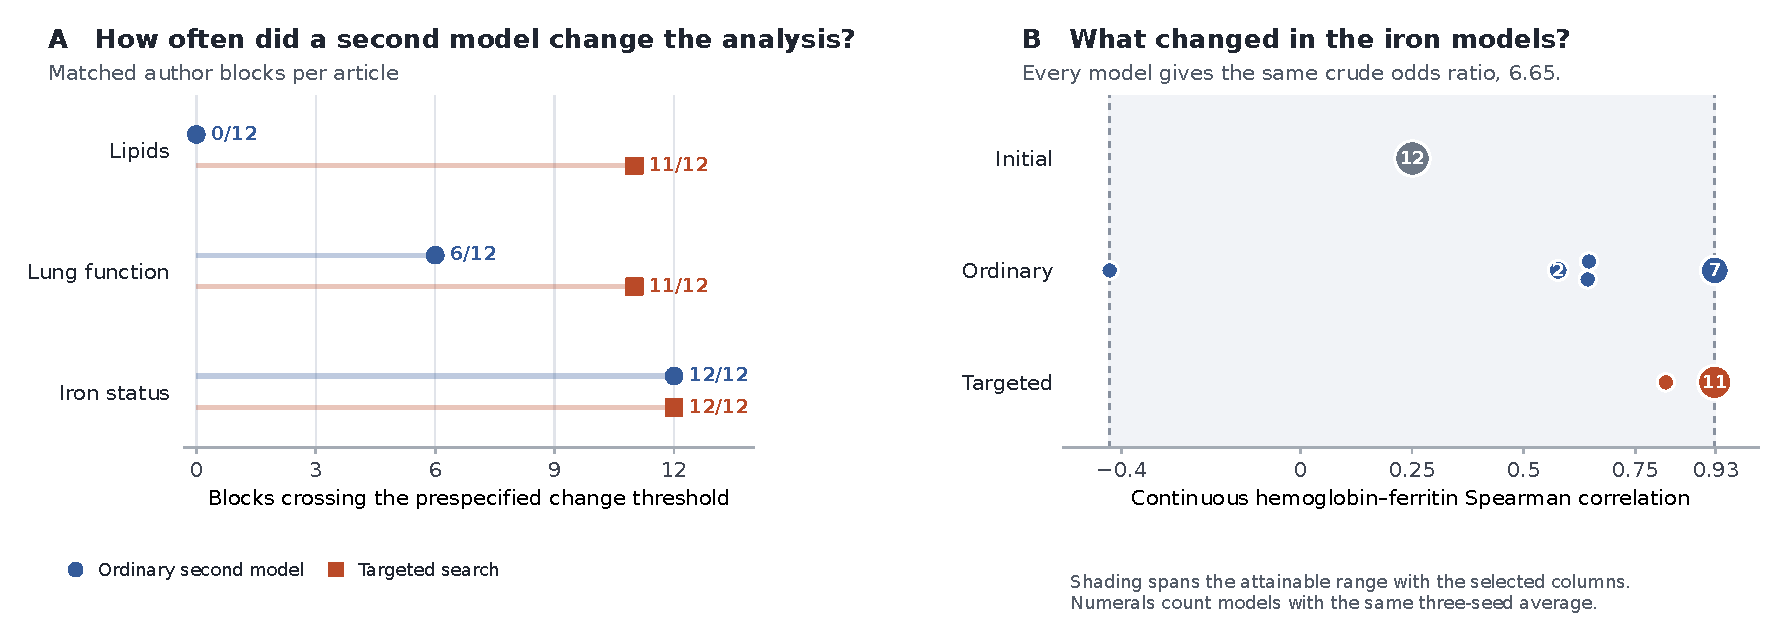
\includegraphics[width=.96\textwidth]{figures/article-comparison.pdf}
\caption{Left: ordinary and targeted follow-ups to the same initial program. Twelve assigned blocks per article enter each denominator. Right: all 36 iron programs retain the same four threshold counts. Rank correlation varies with the assignment of ferritin to hemoglobin. Shading gives the interval between the two attainable extrema for the fixed columns and bands, computed after scoring.}
\Description{Material changes occur in zero versus eleven lipid blocks, six versus eleven lung blocks, and twelve versus twelve iron blocks. In iron, all twelve initial programs produce the same rank correlation, while feasible assignments under the numerical constraints give correlations of both signs.}
\label{fig:matchedarticles}
\end{figure*}

\paragraph{Screening prevalence.}
For lipids, the ordinary request yielded a material change in 0/12 blocks. The targeted request did so in 11/12 (paired exact $p=0.00098$). The median absolute change rose from 0.27 to 13.18 percentage points. Every accepted pairing preserved mean non-HDL at 128.77~mg/dL. Figure~\ref{fig:lipidlead} illustrates why these two estimates behave differently using a separate four-author experiment on the same source. Each author supplied two admissible assignments; their screening gaps ranged from 16.37 to 29.35 points. A numerical solver subsequently exhibited feasible rates of 9.375\% and 41.406\%. These pairs demonstrate possibilities under the chosen columns; their frequency among real populations is unknown.

\paragraph{Lung function.}
Six ordinary and eleven targeted follow-ups out of twelve attained the registered change in the proportion below an individual FEV$_1$/FVC of 0.70 ($p=0.0625$). An audit after scoring found a median 15.28\% of the targeted records within 0.005 of the cutoff, compared with 2.63\% under the ordinary request. The agent found ways to move the screening result by concentrating records near a decision boundary. Source agreement alone gives little grounds to expect that concentration in practice. A separate deterministic solver constructed two admissible rates of 1.18\% and 52.46\% while retaining the 76.24\% ratio of means.

\paragraph{Iron status.}
All twelve ordinary and all twelve targeted follow-ups materially changed continuous rank correlation. The initial authors had produced exactly the same assignments at shared seeds. Seven follow-up pairs also produced identical assignments in the two arms. Here the threshold bands make two extrema calculable: ordering ranks in opposite or identical order within the permitted bands attains correlations of $-0.427$ and $0.928$ for these finite columns. All 36 programs retain the four threshold counts and therefore the odds ratio of 6.65. The sign of an association between continuous measurements can be open even when a binary association between the same biomarkers is fixed.

\section{Which estimates carry over to measured participants?}
\label{sec:lifestyle}
\subsection{Run the published lifestyle analysis with the data replaced}
Lea et al.~\cite{lea,leadata} compared pastoralist, rural nonpastoralist and urban nonpastoralist Turkana in Kenya. Two agents read the paper, could search for further evidence, and each authored a whole-cohort program containing lifestyle, age, sex, BMI, total cholesterol and HDL. The material described higher urban BMI and total cholesterol and the absence of a detected HDL contrast. The authors chose the magnitudes, within-group variation and covariate relationships. Each program yielded three tables of 1,226 virtual participants. We withheld the measured rows and our fitted coefficients.

\begin{figure*}[t]
\centering
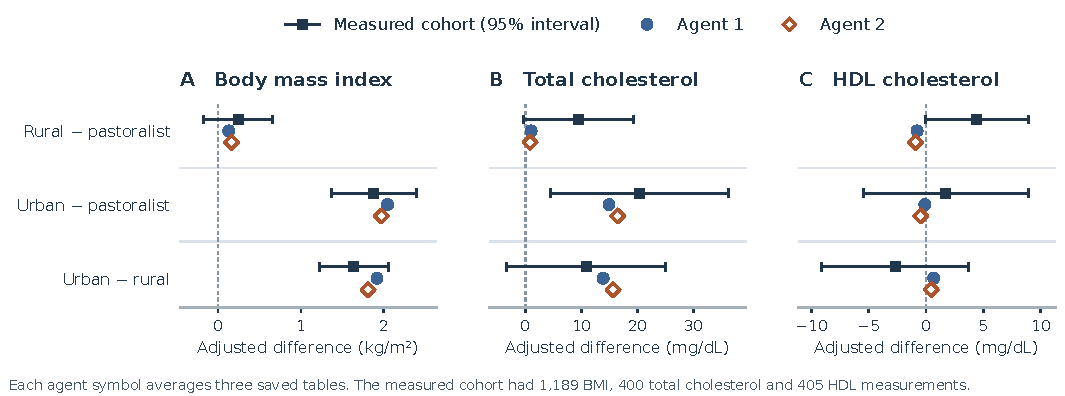
\includegraphics[width=.99\textwidth]{figures/lifestyle-effects.pdf}
\caption{Only the analysis input changes. Squares give adjusted lifestyle contrasts on measured participants and pointwise 95\% OLS intervals. The two other symbols are means over the three draws of each agent-authored generator. All nine prespecified pooled contrasts are shown in the original measurement units. Each panel has its own scale.}
\Description{Three panels show rural minus pastoralist, urban minus pastoralist, and urban minus rural effects. Both virtual cohorts track positive urban BMI contrasts. Urban total cholesterol remains higher but below the measured point estimate. HDL estimates in both virtual cohorts stay near zero.}
\label{fig:lifestyle-main}
\end{figure*}

We implemented the published age- and sex-adjusted three-group regression once and changed only its input. The original analysis code was unavailable. The measured available-case samples contained 1,189 people for BMI, 400 for total cholesterol and 405 for HDL. Figure~\ref{fig:lifestyle-main} displays all nine prespecified pooled contrasts. The appendix retains the sex-specific and interaction analyses (Appendix~\ref{app:lifestyle}).

Measured urban participants had an adjusted BMI 1.88~kg/m$^2$ higher than pastoralists (95\% interval 1.37--2.40). The two virtual estimates were 2.05 and 1.97. Two matched resamples of real participants differed by 0.316~kg/m$^2$ on average in absolute value. The corresponding virtual--real discrepancy ranged from 0.314 to 0.428. For urban total cholesterol, the measured elevation of 20.34~mg/dL became 14.96 and 16.53~mg/dL. Standardizing by each table's own SD obscured this attenuation because the virtual distributions were narrower. For rural versus pastoralist total cholesterol, the measured contrast was 9.49~mg/dL (95\% interval $-0.37$ to 19.36); the virtual estimates were 1.06 and 0.87. A reader planning a cholesterol study needs these effects in mg/dL.

\subsection{Separate the agent's contribution from the group structure}
\label{sec:chns}
We re-paired age with the intact biomarker vector within each sex and lifestyle group in each frozen Kenyan table. The expected urban--pastoralist BMI contrast shifted by just 0.0025--0.0110~kg/m$^2$, small beside 0.316 under real resampling. The supplied group structure accounts for much of the reproduced BMI comparison. This was a retrospective attribution check (Figure~\ref{fig:attribution}).

\begin{figure*}[t]
\centering
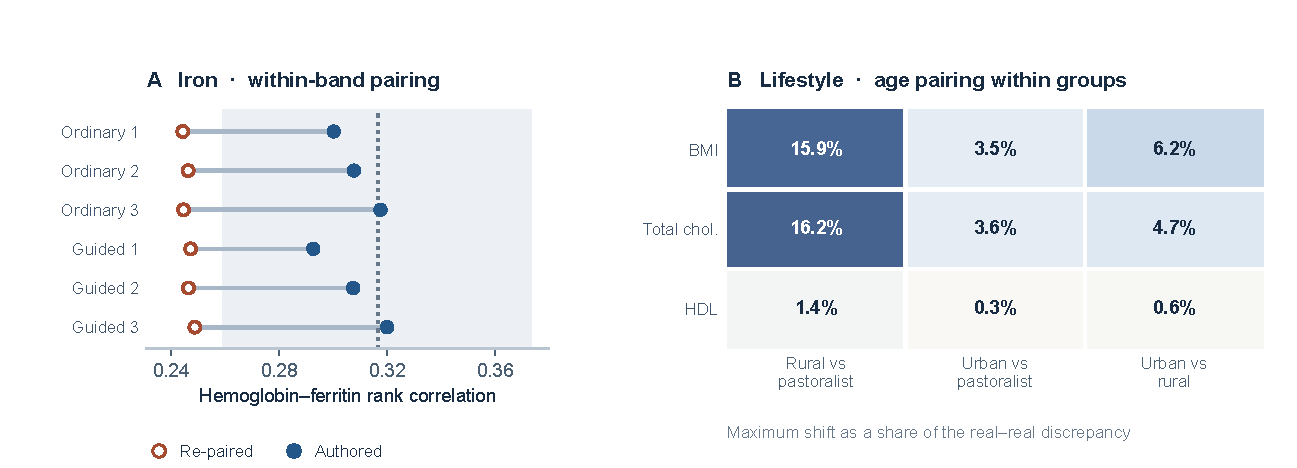
\includegraphics[width=.94\textwidth]{figures/pairing-attribution.pdf}
\caption{How much of an analysis comes from the agent's pairing? (A) Each line follows one CHNS law from the expected correlation after randomly re-pairing within Hb bands to its authored value. The dotted line and shading show the measured correlation and its 95\% interval. (B) In the lifestyle case, age was re-paired with the intact biomarker vector within sex and lifestyle groups. The cells show the largest absolute change over all six virtual tables as a percentage of the mean absolute difference between two real resamples for that regression. These are retrospective within-table comparisons.}
\Description{All six authored iron correlations lie closer to the measured sample than their re-paired counterparts. The largest age-pairing shift for the nine lifestyle regressions ranges from 0.3 to 16.2 percent of the corresponding real resampling discrepancy.}
\label{fig:attribution}
\end{figure*}

A community holdout in the China Health and Nutrition Survey (CHNS) gave a different result~\cite{chnsbio,chnsind}. The authors received an iron article, threshold counts and band summaries from 1,123 women in 110 communities. A disjoint set of 1,082 women in 107 communities supplied the reference. Re-pairing the two biomarkers within hemoglobin bands kept each agent's own bandwise distributions. Restoring the authored pairing moved all six original-evidence correlations closer to the measured estimate, reducing absolute error by a median of 0.0612. The threshold odds ratio remained invariant. This within-table comparison was specified after disclosure.

In a paired revision experiment the agent also received a local ferritin contrast in one hemoglobin band. Five of six revisions improved agreement with that supplied contrast. Only one improved the held-out whole-sample rank estimate. The final six correlations spanned 0.297--0.304 against a measured 0.317 (95\% community-bootstrap interval 0.259--0.373). The six crude odds ratios were 4.990--5.124 against 4.218 (2.979--6.042). The original threshold table already implied 5.083. These results support the two registered planning tolerances at the measured points; improvement on the local statistic had limited bearing on the global analysis (Appendix~\ref{app:chns}).

\subsection{Freeze the pairing before examining another population}
\label{sec:gripmain}
An Australian study reports separate left- and right-hand grip summaries by sex and age~\cite{grip_adelaide}. We asked for the mean absolute difference between the hands of the same adult. Four agents chose a Gaussian dependence model with correlation 0.80. Applied to the same single-hand values, independence predicted 7.93~kg and the authored pairing predicted 3.81~kg. We froze both before opening the US and rural South African participant pairs~\cite{grip_cdc,grip_haalsi}. The standardized means were 3.30~kg (95\% interval 3.07--3.52) and 3.78~kg (3.52--4.05). The reduction in error exceeded the registered 1~kg criterion in both settings. The four authors supplied one numerical hypothesis. For the additional question of a gap of at least 5~kg, its estimate of 28.94\% was closer to rural South Africa (27.71\%) than to the US (20.95\%). Appendix Figure~\ref{fig:gripgroups} gives the full threshold sweep and subgroup checks.

In Akwa Ibom, Nigeria, we prospectively compared six agents with a statistical generator that could also fit dependence within a band. Every constructor received the same Chinese article, the same CHNS summaries and the same fixed columns. Each agent selected a Gaussian rank copula calibrated in the middle band and extended it across bands. Five produced byte-identical assignments at shared seeds. The statistical generator predicted an overall rank correlation of 0.303, and the median agent prediction was 0.308. The 603 measured mothers had a correlation of 0.010 (95\% interval $-0.064$ to 0.086). Both arms gave a threshold odds ratio of 5.39, compared with 1.20 (0.71--1.90) in the reference. Neither met the registered transport criteria (Appendix~\ref{app:akwa})~\cite{akwa_iron}. What looked like agreement among independent sessions was agreement on one extrapolation.

\section{Related work}
\paragraph{Constructing records from summaries.}
SynthIPD reconstructs survival data with covariates, and KMGen extracts survival curves and combines evidence with a mechanistic patient model~\cite{synthipd,kmgen}. Patient-Zero builds patient records from medical knowledge~\cite{patientzero}. Text2Tabular extracts statistics from papers, fits a copula and uses constrained sampling to incorporate reported test results. Its evaluation pairs published papers with their original tables~\cite{gottal2026text2tabular}. LLMSynthor infers dependence and refines records against target summaries, and G-Sim uses language models to design and calibrate simulators~\cite{llmsynthor,gsim}. Other systems address clinical synthesis and virtual lipid populations~\cite{synthcraft,allenlipid,fasseeh}. These methods motivate our same-information control. Once two generators match the reported evidence, we ask the agent to exhibit what their agreement leaves unresolved for one specified scientific analysis.

\paragraph{Dependence and analysis-specific utility.}
Statistical reconstruction methods can recover an ANCOVA estimate from suitable trial summaries or infer regression inputs from a reported correlation matrix~\cite{pseudoancova,bonofiglio}. Fixed marginals and additional moments restrict the space of joint laws~\cite{bounds,makarov,zaev}. Snoke et al.\ distinguish utility for a specified analysis from general distributional resemblance~\cite{specificutility}. Azizi et al.\ repeat a published analysis on partially synthesized trial records, and Decruyenaere et al.\ assess generators across 115 oncology trials~\cite{azizi,oncology115}. Our comparison retains the scientific estimator and manipulates one authoring decision. It can attribute a change in an estimated screening fraction to a particular permutation of the same measurements.

\section{Discussion}
The strongest evidence for an agent contribution is an executable alternative. For cholesterol the agent produced assignments that preserve both marginal columns and the reported ratio, yet give materially different screening counts. For iron one can go further and calculate the extreme correlations allowed by the finite columns. A deterministic solver can also find admissible counterexamples. The matched experiment measures what the agent can uncover when a researcher asks for one; it leaves the relative efficiency of search algorithms open.

A second experiment is necessary to decide whether a specific assignment can support a real use. The relevant comparisons retain the units of each research question: a hand difference in kg, a cholesterol contrast in mg/dL, or a rate per hundred people screened. The paired grip model substantially improved the mean difference in two external samples. The same approach to extending one source-band relationship to a different population produced excessive iron dependence in Nigeria. The source evidence, published constraints, and independent checks answer different parts of the researcher's question.

The matched trial covers three reused articles and one GPT configuration. It demonstrates attainable differences under specified marginals, without assigning probabilities to the alternatives. Kenya evaluates a published result in its source population, CHNS separates communities in one survey, and the Brazilian blood-pressure and US iron references had been used during development. Appendix~\ref{app:ocular} includes a successful held-out eye-pressure threshold and a BMI underreporting threshold that all six assigned sessions missed. A useful release can therefore identify, for each requested analysis, the evidence that constrains it, the author's remaining choice, and the available population comparison.
\bibliographystyle{ACM-Reference-Format}
\bibliography{references}
\clearpage
\appendix
\section{Construction, data and reproducibility}
\label{app:design}
\begin{table}[htbp]
\caption{Measured comparisons by scientific use. Each entry represents a recruitment sample or survey period for that analysis.}
\label{tab:scope}
\small\centering
\begin{tabular}{@{}lrp{.53\columnwidth}@{}}
\toprule
Analysis & Samples & Measured settings\\
\midrule
Lifestyle & 1 & Kenyan Turkana\\
Blood pressure & 2 & Brazil PNS, Freetown\\
Iron status & 4 & US NHANES, Burkina Faso, Chinese communities, Nigeria\\
Lipids & 5 & Two Ethiopian studies, Virginia, two US national survey periods\\
Handgrip & 3 & US NHANES, rural South Africa, Rio Branco (maximal trials)\\
Spirometry & 2 & US NHANES, rural Malawi (first follow-up)\\
\bottomrule
\end{tabular}
\end{table}

\paragraph{Original papers.}
All six original-paper constructors used the requested and returned model identifier \texttt{gpt-6.1-sol}. Each had a fresh context and access to the task, the assigned article, supplementary search, the sampler contract and the generated-only inspection tool. The program, declared parameters and provenance notes were sealed before target comparison. The three final sampling seeds were 17121, 17123 and 17127. Each pressure draw had 3,000 rows and each iron draw 5,000. Estimators were also implemented independently using regression, counts and ranks. A target-family search preview in one pressure session contained survey identity, demographics and a qualitative topic. The session recorded and excluded it. The target slopes and paired correlation were withheld.

\paragraph{Pressure reference.}
The PNS operator uses the positive laboratory survey weight in a complete-case frame aged 20--79. It excludes recorded pregnancy. Unknown pregnancy status is retained under the frozen rule. The same rows enter both regressions. The design matrix contains an intercept, age, recorded sex and BMI in units of five kg/m$^2$. We correlate the residuals of the two pressure models. Synthetic records receive equal weights because the requested generator targets the weighted distribution. Five hundred row resamples retaining the survey weights gave conditional stability intervals of [2.96, 4.12] for the systolic slope, [1.93, 2.59] for the diastolic slope and [0.700, 0.734] for the residual correlation. The released workbook did not support a design-based cluster variance calculation.

\paragraph{Iron reference.}
NHANES August 2021--August 2023 supplies the measured hemoglobin, ferritin and survey-design variables. The eligible sample contains 979 nonpregnant women aged 20--44 with both measurements and positive phlebotomy weights. The frozen analysis uses raw ferritin with no inflammation adjustment. The three estimators are the weighted four-cell odds ratio, the weighted fraction with both markers low and a weighted Spearman correlation. A stratified delete-one-primary-sampling-unit calculation with 15 strata and 30 primary sampling units gave 95\% intervals of [9.28, 34.11] for the odds ratio, [6.07, 9.55]\% for both markers low and [0.318, 0.473] for the rank correlation.

\paragraph{Controlled evidence.}
The pressure and iron controls used nine fresh constructors each, with three seeded draws per constructor. The source block was masked before the modeling call. For pressure this hid or revealed six same-sample entries relating SBP, DBP, BMI and age. For iron it hid or revealed a paired contingency table. Neither experiment supplied the desired target result. The common base differed between cases, so cross-case comparisons of the base arm do not measure a shared zero-information condition. Both experiments used one model call per constructor, no feedback round and the same GPT identifier as the original-paper trials. Usage valued at the recorded tariffs was US\$0.92 for pressure and US\$0.68 for iron.

\paragraph{What orchestration adds.}
A separate developmental comparison started both an ordinary coding agent and a structured workflow from a research request. They had the same GPT model, search and runtime capabilities, and resource limits. Across 12 constructions and 36 seeded tables, the ordinary agent had smaller mean absolute discrepancies on four of the six focal analyses and the structured workflow on two. This result supports using a simple agent as a viable constructor. The source-to-code records serve the separate purpose of making each scientific choice inspectable.

\paragraph{Use of generative AI.}
The construction experiments used the model recorded above. OpenAI Codex also assisted in drafting the English manuscript, preparing the \LaTeX{} files and checking reported numerical results against the experimental artifacts.

\section{CHNS holdout, paired evaluation and local decomposition}
\label{app:chns}
\begin{figure*}[t]
\centering
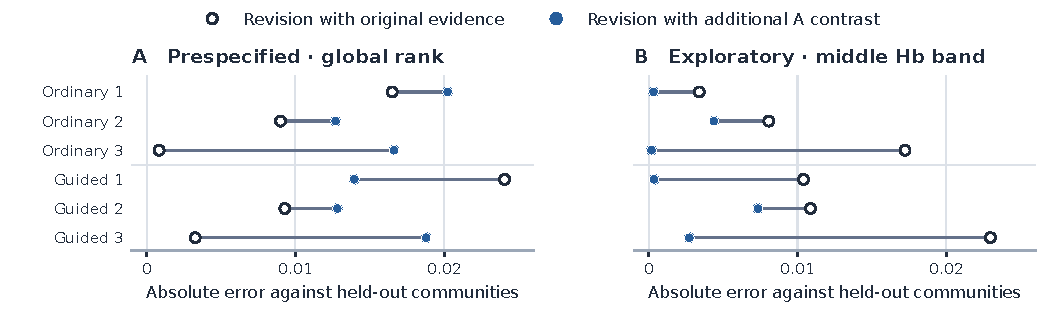
\includegraphics[width=.98\textwidth]{figures/chns-revision.pdf}
\caption{What changed when a constructor received one extra conditional contrast? Each row pairs two revisions of the same parent. Leftward movement means smaller absolute error against CHNS B. (A) On the prespecified whole-cohort rank correlation, one of six moves closer. (B) In a post hoc decomposition, all six move closer on the middle Hb band's weighted contribution to the global correlation. The two panels use the same scale. The B reference is a sample estimate.}
\Description{Paired error plots for three ordinary and three workflow constructors. Additional evidence lowers whole-cohort rank error for the first workflow constructor. It reduces the error in the middle-band contribution for every constructor.}
\label{fig:revision}
\end{figure*}
\paragraph{Population.}
We linked 2,218 age-eligible women with the required survey fields. Of these, 2,205 had positive paired measurements. We converted the central Hb field from g/L to g/dL. Serum ferritin in ng/mL is numerically equal to $\mu$g/L. Ferritin was uncorrected for inflammation. Eligibility included all recorded pregnancy and inflammation statuses. We analyzed complete cases without national survey weights. Estimates describe this sample of women. Within province, a fixed hash ordering assigned alternate communities to A and B. We sealed the split, input hashes, research questions, tolerances and evidence schedule before model calls. The study articles supplied no measurements from B.

\paragraph{Construction.}
Each arm had three initial sessions. We interleaved the sessions and used the same GPT configuration and isolated runtime throughout. Each of the six parent programs had two sealed sibling revisions. One saw the original evidence and the source checks on the parent. The other also saw the added A contrast. All 18 requests returned programs. Each program drew 12,000 records at each of three common seeds. The scientific analysis pooled the three draws per program. The 54 tables are simulation repeats nested within six parents and one survey split. The 18 calls cost US\$1.77 at recorded token tariffs. A separate implementation reproduced the table analyses, the B intervals and both arm decisions before manuscript integration.

We computed Spearman correlation from average ranks for ties. For the crude odds ratio B had 114 both markers low, 116 only Hb low, 161 only ferritin low and 691 neither. The odds ratio is $(114\times691)/(116\times161)=4.218$. All four cells exceeded the minimum of ten. We used 2,000 province-stratified whole-community bootstrap replicates in each half. The B interval for correlation met the prespecified precision rule (half-width at most 0.10). The study's final-use rule required absolute rank error at most 0.10, an augmented odds ratio within a factor of 1.50 of B's, and augmented and control odds ratios within a factor of 1.20 of one another. All six passed. The primary incremental contrast subtracts augmented absolute rank error from control absolute rank error. A material arm-level benefit required all three pairs, median gain at least 0.05 with lower bootstrap limit above zero, at least two final-use passes and sufficient B precision. Conditional on the three parents per arm, the 95\% B-sampling intervals for the median gains were [$-0.0037$, $0.0037$] and [$-0.0035$, $0.0090$] for ordinary and guided sessions, respectively. Neither arm met the rule.

\begin{table*}[t]
\caption{All six CHNS sibling comparisons, with three pooled draws per program. C denotes revision with the original evidence. E denotes its sibling given the additional A contrast. A positive gain is a reduction in absolute error for the whole-cohort correlation. The final two columns describe errors in the probability-weighted middle-band contribution, examined after B was opened.}
\label{tab:chns}
\centering
\begin{tabular}{@{}lrrrrrr@{}}
\toprule
 & \multicolumn{4}{c}{Prespecified whole-cohort analyses} & \multicolumn{2}{c}{Exploratory local error}\\
\cmidrule(lr){2-5}\cmidrule(l){6-7}
Parent & Rank C & Rank E & Rank gain & Odds ratio E & C & E\\
\midrule
Ordinary 1 & 0.3003 & 0.2966 & $-0.0037$ & 5.1149 & 0.0034 & 0.0003\\
Ordinary 2 & 0.3078 & 0.3041 & $-0.0037$ & 4.9900 & 0.0081 & 0.0044\\
Ordinary 3 & 0.3176 & 0.3002 & $-0.0158$ & 5.1224 & 0.0172 & 0.0002\\
Guided 1 & 0.2927 & 0.3028 & $+0.0101$ & 5.0992 & 0.0104 & 0.0004\\
Guided 2 & 0.3075 & 0.3040 & $-0.0035$ & 5.1237 & 0.0109 & 0.0073\\
Guided 3 & 0.3201 & 0.2980 & $-0.0155$ & 4.9924 & 0.0230 & 0.0027\\
\bottomrule
\end{tabular}
\end{table*}

\paragraph{Exploratory covariance partition.}
Let $U,V$ denote global sample midranks of Hb and ferritin, each centered and standardized to unit variance with the full sample denominator. Let $G$ partition Hb at 12 and 14 g/dL. Then
\begin{align*}
\rho_S
  &= \operatorname{Cov}\{\mathbb E[U\mid G],\mathbb E[V\mid G]\}\\
  &\quad +\sum_g \Pr(G=g)\operatorname{Cov}(U,V\mid G=g).
\end{align*}
The middle-band value uses the original global ranks with the band-specific covariance and the band's sample weight. Reranking participants within the middle band would define a different statistic. In B, the between-band term was 0.270538 and the within-band terms were 0.011512, 0.034290 and 0.000460. Their sum gives 0.316800 up to rounding. For Guided 3 the middle contribution changed from 0.05726 to 0.03702 while the global rank correlation moved farther from B. Across parents, the between-band estimates were 0.2444--0.2489 with the original evidence and 0.2444--0.2474 with the extra contrast. Table~\ref{tab:chns} retains both the predeclared endpoints and the six descriptive component comparisons.

\begin{table*}[t]
\caption{What did the CHNS A evidence alone supply? The B reference is a Spearman correlation of 0.3168 and a crude odds ratio of 4.218. All four rows use only the original evidence. The retrospective statistical model and each of the six agent models use 36,000 draws per law. Ranges cover the six original-evidence agents. Re-pairing gives the expected correlation under a uniform permutation within each Hb band and leaves each agent's four threshold counts unchanged.}
\label{tab:chnsattribution}
\centering
\begin{tabular}{@{}lrrrr@{}}
\toprule
 & \multicolumn{2}{c}{Continuous Hb and ferritin} & \multicolumn{2}{c}{Threshold association}\\
\cmidrule(lr){2-3}\cmidrule(l){4-5}
Construction & Spearman $\rho$ & $|\rho-\rho_B|$ & Odds ratio & $|\log(\mathrm{OR}/\mathrm{OR}_B)|$\\
\midrule
Direct A threshold counts & --- & --- & 5.083 & 0.187\\
Statistical model, independent within Hb band & 0.2370 & 0.0798 & 5.023 & 0.175\\
Agent records, expected after within-band re-pairing & 0.2444--0.2489 & 0.0679--0.0724 & 4.998--5.175 & 0.170--0.205\\
Agent records, original pairing & 0.2927--0.3201 & 0.0008--0.0241 & 4.998--5.175 & 0.170--0.205\\
\bottomrule
\end{tabular}
\end{table*}

\paragraph{Incremental effect on the prespecified whole-cohort analysis.}
The revisions using only the original evidence reproduced all 18 initial tables byte for byte at the three shared seeds. Five of six augmented laws came closer to the supplied A contrast on the log scale. In B only one came closer on whole-cohort rank correlation (Figure~\ref{fig:revision}A). Median reductions in absolute rank error were $-0.0037$ for ordinary and $-0.0035$ for guided constructors. The prespecified material gain was 0.05. The largest control error against B was 0.024, already below that benchmark. Even a perfect revision at the observed B estimate could therefore have gained at most 0.024.

For the middle-band within-group contribution, median absolute error fell from 0.01064 to 0.00155. Errors in this component and the between-band component could offset one another. Table~\ref{tab:chns} gives the individual comparisons.

\subsection{A statistical model using the original CHNS evidence}
\label{app:chnsstat}
The retrospective comparator uses the same evidentiary inputs as the six original-evidence parents. The Zhu article supplies the scientific context and definitions. The A tables give numerical constraints in the survey population, so we use their counts and moments wherever the sources overlap. The model was specified after B was public. We recorded its equations, source hierarchy, scoring code, seeds and input hashes before scoring its draws. This compares statistical constructions given extracted evidence. It does not test article retrieval or extraction.

Let $G$ denote the three Hb bands. The model samples $G$ with probability $n_g/1123$. Conditional on $G$, it samples Hb and ferritin independently. For Hb we fit a beta distribution by moments on $(0,12)$ or $(12,14)$ and a shifted gamma law above 14. For $Y=\log(\mathrm{ferritin})$ we use the maximum-entropy density subject to the reported log mean, log variance and probability below $k=\log 15$. It has the form
\[
q_g(y)\ \propto\ \exp\{a_g y+b_g y^2+c_g\,\mathbf{1}_{y<k}\},\qquad b_g<0 .
\]
This is a normal density reweighted on either side of $k$. We set the two masses using the reported depletion frequency and solve for the underlying normal location and scale by matching the two log moments. At the resulting solution, every competing density satisfying the constraints has the same expectation of $\log q_g$. Nonnegativity of relative entropy then gives the stated entropy maximum on the log scale. This is one choice of marginal family and one assumption about dependence. Numerical integration verified all three fitted probabilities, means and dispersions against the A tables.

For the analytic population rank let $w_g=\Pr(G=g)$, $u_g=\sum_{j<g}w_j+w_g/2$, and $F_Y$ be the mixture CDF of log ferritin. Since the Hb bands are ordered and the two markers are independent within a band, $\rho_S=12\sum_g w_g u_g \mathbb E[F_Y(Y)\mid G=g]-3$. Integration gives 0.2414 and the four source cells give an OR of 5.083. The three 12,000-row draws gave ranks of 0.2456, 0.2451 and 0.2198. Pooling the records with the original estimator gives Table~\ref{tab:chnsattribution}. Direct per-draw rank and cell calculations reproduced both endpoints. The comparison uses zero additional model calls.

The re-pairing row uses the existing agent records. Under a random permutation of ferritin within each Hb band, the expected within-band covariance of the standardized global midranks is zero. All ranks and the number of threshold crossings per band retain their original marginal values. The between-band covariance in the preceding decomposition is therefore the exact expected Spearman correlation under that permutation. Table~\ref{tab:chnsattribution} reports its distance from B's estimate. The paired absolute-error reductions from the authored pairing ranged from 0.0454 to 0.0713. This is a conditional comparison on the six saved laws; the three seeds per law approximate that law's output.

\section{Every original-paper outcome}
\label{app:profiles}
\begin{figure*}[t]
\centering
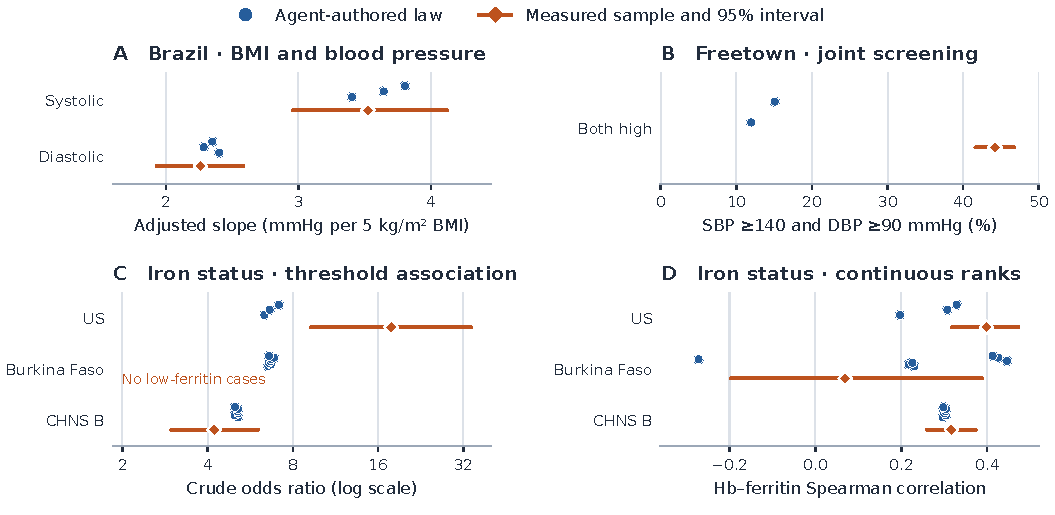
\includegraphics[width=.98\textwidth]{figures/analysis-support.pdf}
\caption{What the virtual cohorts support when the scientific analysis stays fixed. Each circle is one agent-authored law. Diamonds and bars show measured estimates and their 95\% intervals. (A) Three constructors recover the scale of the adjusted Brazilian blood-pressure slopes. (B) Two laws that share five source moments both understate the joint screening rate in the deposited Freetown fields. (C, D) Each iron cohort supplies both a threshold odds ratio and a continuous rank correlation. Burkina Faso has no low-ferritin cases. In CHNS the six final laws meet both prespecified planning tolerances. Brazil and the US are development comparisons. Freetown and Burkina Faso are external assessments. CHNS B comprises communities held out within a survey. The Brazilian bars describe row-resampling stability.}
\Description{Four panels compare modeled and measured quantities in their native units. Blood-pressure slopes are close in Brazil. The Freetown joint rate is much higher in the release. Iron models preserve the source odds ratio in the US and Burkina Faso tasks while continuous ranks vary. Both CHNS analyses show positive associations near the held-out estimates.}
\label{fig:support}
\end{figure*}

\begin{figure*}[t]
\centering
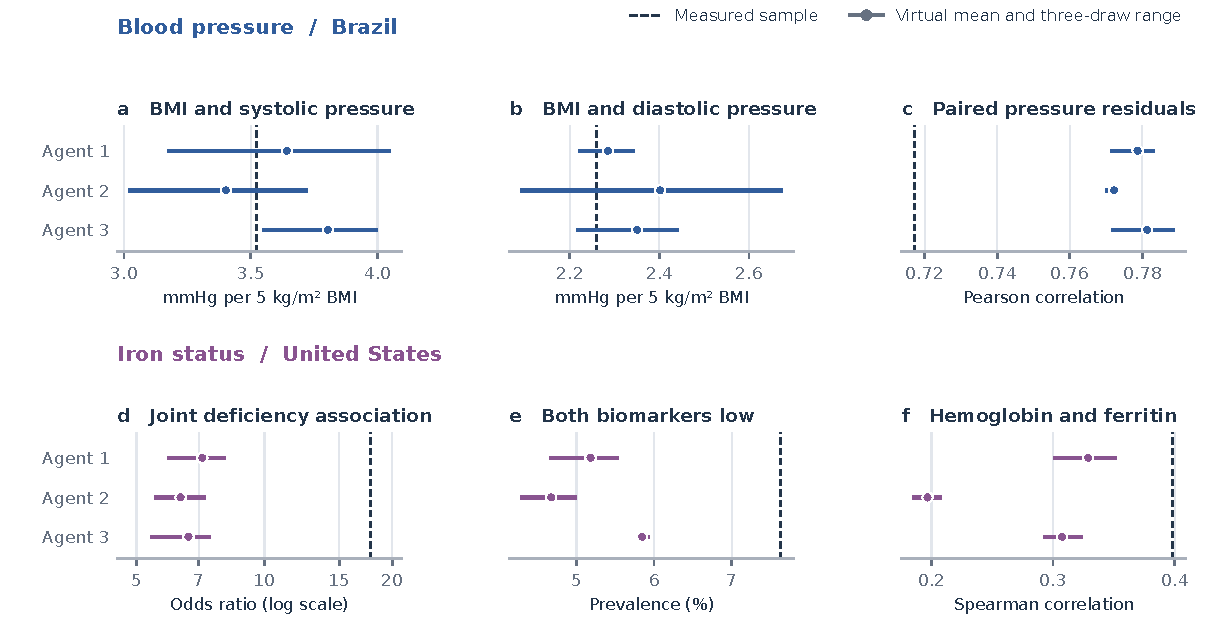
\includegraphics[width=.85\textwidth]{figures/original-paper.pdf}
\caption{The same analysis run on virtual and measured records. Each point is one constructor's mean across three seeded draws. The segment spans those draws. Dashed lines are measured sample estimates. Each panel has its own scale. The systolic slopes are near the Brazilian estimate. The iron odds ratios cluster around the value derived from the Chinese source paper, well below the US estimate.}
\Description{Six panels compare three constructors with a measured reference. The three systolic slopes straddle the reference, all diastolic slopes and residual correlations exceed it, and all three iron odds ratios, joint prevalences and rank correlations fall below their reference.}
\label{fig:original}
\end{figure*}

Table~\ref{tab:profile} preserves all three primary endpoints and the accompanying diagnostics in each case. Author numbers identify independent sessions within one task. The zero ordering violation rate follows from the positive pulse-pressure construction. Across the iron sessions, the two marginal deficiency fractions move in opposite directions relative to the US sample. The isolated threshold odds ratio is therefore an incomplete guide to biomedical utility.

\begin{table}[htbp]
\caption{All original-paper estimates. A1--A3 are constructor means over three seeded draws. The final column is the measured sample. Percentages use a 0--100 scale.}
\label{tab:profile}
\centering
\begin{tabular}{@{}lrrrr@{}}
\toprule
Analysis & A1 & A2 & A3 & Measured\\
\midrule
\multicolumn{5}{@{}l}{\emph{Brazilian blood pressure}}\\
BMI--SBP slope & 3.642 & 3.402 & 3.804 & 3.524\\
BMI--DBP slope & 2.285 & 2.402 & 2.350 & 2.260\\
Residual correlation & .779 & .772 & .781 & .717\\
SBP SD (mmHg) & 20.00 & 19.70 & 19.57 & 18.19\\
DBP SD (mmHg) & 11.57 & 11.57 & 11.47 & 11.09\\
SBP $<$ DBP (\%) & 0 & 0 & 0 & 0\\
\midrule
\multicolumn{5}{@{}l}{\emph{US iron status}}\\
Threshold odds ratio & 7.141 & 6.348 & 6.625 & 17.790\\
Both low (\%) & 5.180 & 4.673 & 5.847 & 7.630\\
Spearman correlation & .329 & .197 & .307 & .398\\
Low hemoglobin (\%) & 10.660 & 8.807 & 11.727 & 15.240\\
Low ferritin (\%) & 15.680 & 18.513 & 17.487 & 12.153\\
\bottomrule
\end{tabular}
\end{table}

\section{Two blood-pressure laws under the same constraints}
\label{app:freetownaccount}
\label{sec:prospective}
\label{app:laws}

\begin{figure*}[t]
\centering
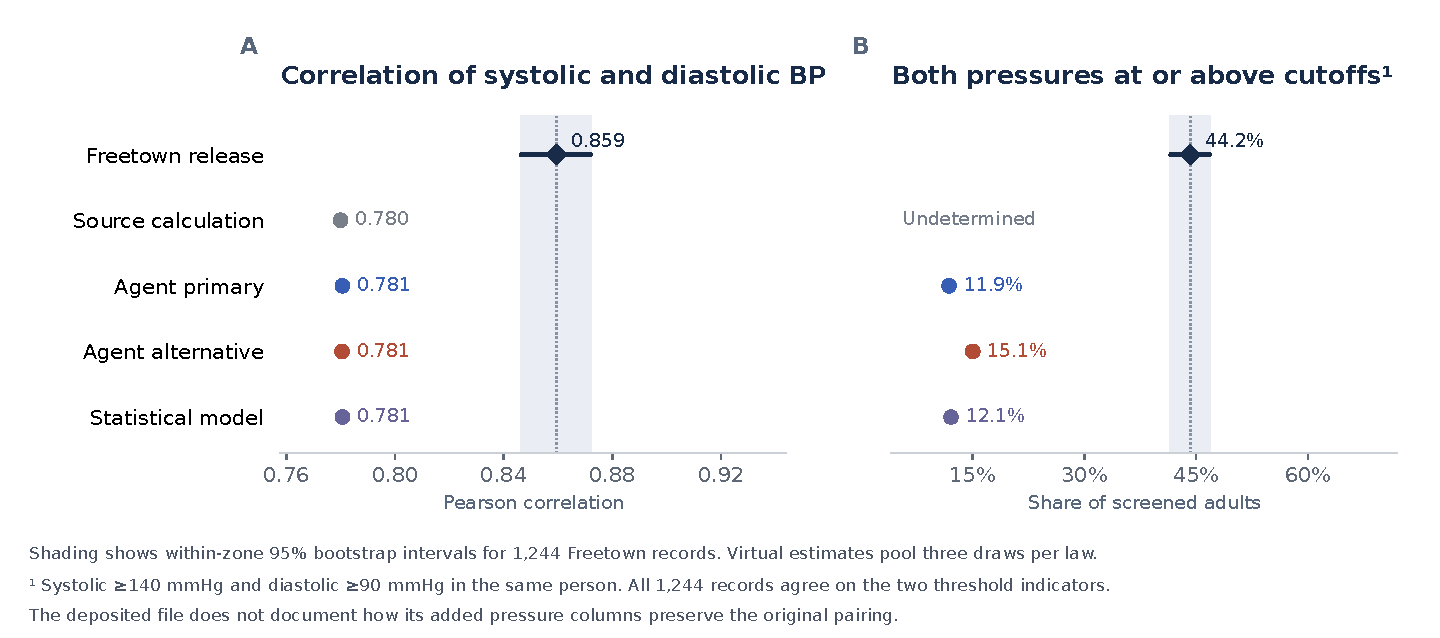
\includegraphics[width=.84\textwidth]{figures/freetown.pdf}
\caption{Prospective screening test. The source correlation is available by direct calculation. The joint threshold probability depends on the model. Points for the two agent laws and the statistical comparator are estimates from seeded virtual draws. The band describes uncertainty for the deposited Freetown sample conditional on the represented zones. The extreme target threshold result led to a separate audit of the deposited fields.}
\Description{Two panels show a released correlation of 0.859 and a joint threshold percentage of 44.2. Three virtual arms give correlations near 0.78 and threshold percentages between 11.9 and 15.1.}
\label{fig:freetown}
\end{figure*}

Let $S$ and $D$ be systolic and diastolic pressure. Write $G=S-D$ for the pulse-pressure gap. From the five source statistics, calculate
\begin{align*}
\mathrm{E}[G] &= \mathrm{E}[S]-\mathrm{E}[D],\\
\mathrm{Cov}(D,G) &= \mathrm{Cov}(S,D)-\mathrm{Var}(D),\\
\mathrm{Var}(G) &= \mathrm{Var}(S)+\mathrm{Var}(D)-2\mathrm{Cov}(S,D).
\end{align*}
The primary program draws positive $(D,G)$ from a bivariate lognormal distribution with these moments. For a vector of positive means $m$ and covariance $V$, the log covariance entries are $\log(1+V_{ij}/(m_i m_j))$ and the log means are $\log m_i$ minus half the corresponding log variance. Here the resulting matrices are positive definite. Setting $S=D+G$ enforces the intended ordering in every row.

The alternative program assigns probabilities 0.75 and 0.25 to components with means $(S,D)=(116.22,76.54)$ and $(152.22,92.54)$ mmHg. In $(D,G)$ coordinates, each component receives a common within-component covariance equal to the required total covariance minus the covariance of the component means. By the total covariance identity this gives the same unconditional first and second moments. The component probabilities and offsets are modeling choices. Conditional-normal quadrature for the event $\{D\geq90,\ D+G\geq140\}$ gives the prospective screening probabilities reported below. Moments alone do not select either law.

\paragraph{Pre-disclosure design and measurement.}
The team screened eligibility, headers, uniqueness, measurement methods and field completeness before fixing the Freetown analysis. The target release identity and outcomes were withheld from the constructor. The primary, alternative, comparator, judgments and integration results were recorded before inspecting the measured joint outcomes. Construction took one recorded GPT call (US\$0.0845 at the recorded tariff). Each law generated three equal-sized draws of 10,000, including three for the independently implemented statistical comparator. The source protocol averaged the last two of three seated readings after at least 15 minutes' rest. Freetown averaged two readings following 3--5 minutes of rest. The source selected partnered rural adults, whereas the target was an urban community screening sample.

The Freetown reference uses paired positive recorded pressure values in prespecified age categories covering adults 40 and older. We computed an unweighted sample correlation and exceedance fraction. Intervals use 2,000 bootstraps of participants within eight zones, conditional on those zones. Across the full release, the audit counted 871 records meeting both thresholds, 1,523 meeting neither and zero in either discordant cell. These counts refer to deposited values. Field-level provenance would be needed to explain the pattern.



\subsection{The prospective Freetown comparison}
Before inspecting paired outcome values in a new Freetown screening release~\cite{freetown,freetowndata}, we specified two analyses: the unadjusted Pearson correlation of SBP and DBP, and the fraction simultaneously reaching 140 mmHg systolic \emph{and} 90 mmHg diastolic. The latter is a conjunction of two thresholds. It has a different interpretation from a clinical hypertension diagnosis. The agent received five rounded source summaries from the rural Burkina Faso study~\cite{jaspert}, comprising means 125.22 and 80.54 mmHg, standard deviations 18.22 and 10.98 mmHg, and raw correlation 0.78. It also received the target sampling context. This experiment starts from extracted summaries. The earlier experiments in Section~\ref{sec:original} test original-paper reading.


One fresh agent was asked to propose a primary and an alternative law and state which analyses the source constrained. Before disclosure, it identified the correlation as reported, the joint threshold as underdetermined and the application to a new population as uncertain. Its primary model coupled positive DBP and pulse pressure with a bivariate lognormal law. A statistical comparator specified in advance from the same five numbers independently used this family. The agent's alternative was a 75:25 mixture. It separated the component means and subtracted their between-component contribution from the within-component covariance. These are hypothetical population structures. Both laws preserve all five working moments, including an exact population correlation of 0.780.

Independent numerical integration of the fixed programs gave joint threshold probabilities of 11.9449\% and 15.0851\%. These two examples establish a 3.14 percentage-point difference consistent with the five summaries. They give a lower bound on the range of answers permitted by those constraints. The full range may be wider. A separately prespecified finite-draw criterion asked whether the simulated gap, after subtracting four times the sum of Monte Carlo standard errors, exceeded two percentage points. The adjusted gap was 1.60 points, below the criterion. We report both results because they answer different questions.

After the freeze we analyzed the deposited fields of 1,244 eligible screening participants aged 40 or older. Their correlation was 0.859 (within-zone bootstrap 95\% interval 0.847--0.872), and 44.21\% met both thresholds (41.64--46.79\%). All three simulated arms were far below the released joint rate (Figure~\ref{fig:support}B and Appendix Figure~\ref{fig:freetown}). A post-disclosure count clarified how to interpret that difference. Of the eligible records, 550 met both thresholds, 694 met neither, and neither isolated exceedance occurred. The same pattern held across all 2,394 released records. The codebook identifies the component fields as added variables. Their pairing history remains unresolved. The measured discrepancy applies to the deposited fields. The unresolved pairing limits its biological interpretation.

\section{Original-paper iron construction and verification}
\label{app:ironpros}
\label{sec:ironpros}

\begin{figure*}[t]
\centering
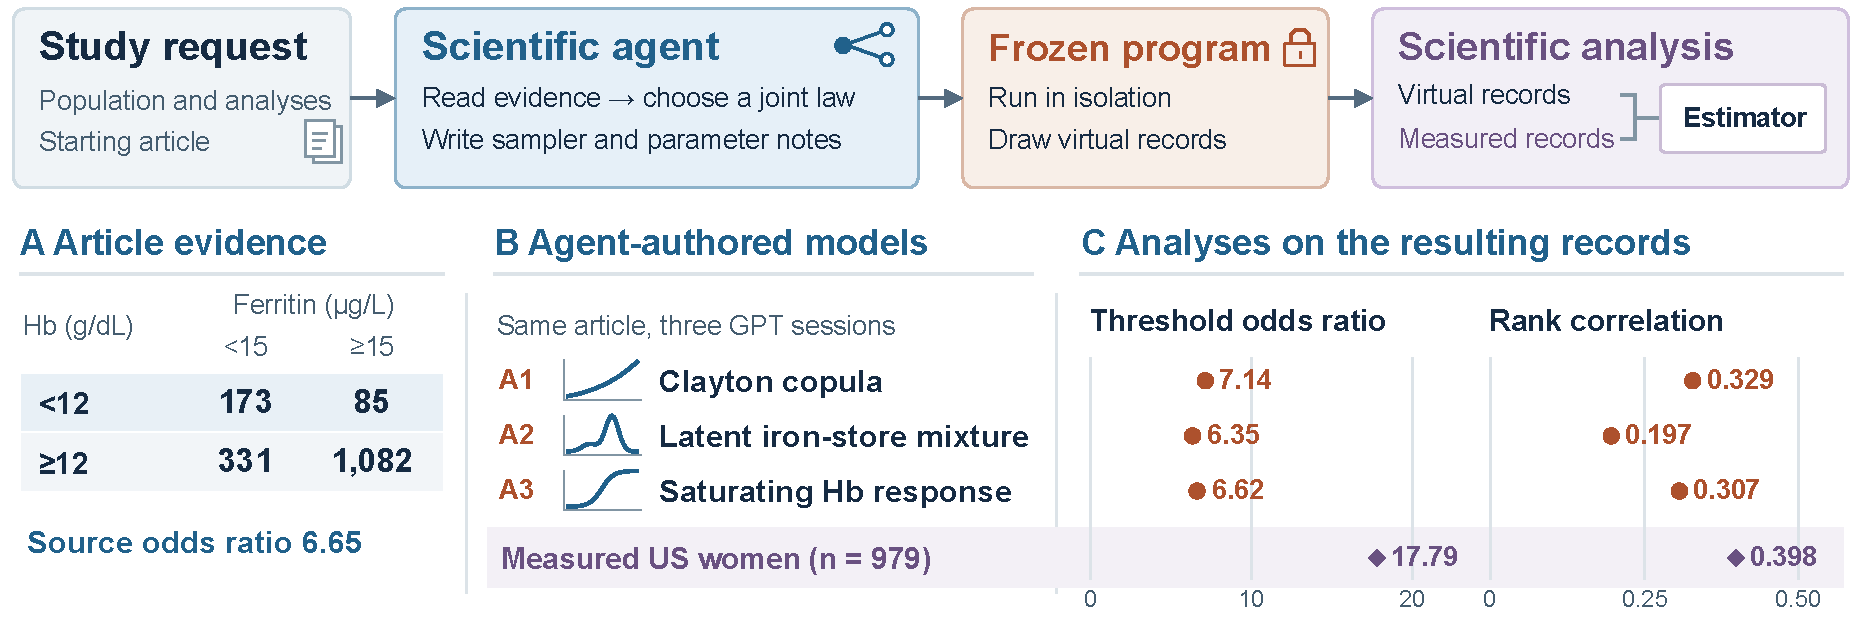
\includegraphics[width=\textwidth]{figures/agent-model-authorship.drawio.pdf}
\caption{From an article to a scientific analysis. The researcher specifies the task. The agent reads the article, chooses a probability law, and writes a sampler that an isolated service executes. In the iron example, three sessions using the same GPT recovered the same source counts from Zhu et al.~\cite{zhu}. Each wrote a different joint model. The small curves show a copula diagonal, latent-store density, and hemoglobin (Hb) response term on separate scales. Orange points average three draws per program. Diamonds show the survey-weighted estimates for 979 US women. All three programs recover the direction of the threshold association and underestimate its measured magnitude.}
\Description{A four-stage diagram traces the request through the scientific agent and frozen program to one analysis of virtual and measured tables. The source odds ratio is 6.65. Three agent-authored models produce odds ratios 7.14, 6.35 and 6.62 and rank correlations 0.329, 0.197 and 0.307. The measured odds ratio is 17.79 and the rank correlation is 0.398.}
\label{fig:method}
\end{figure*}

\begin{figure*}[t]
\centering
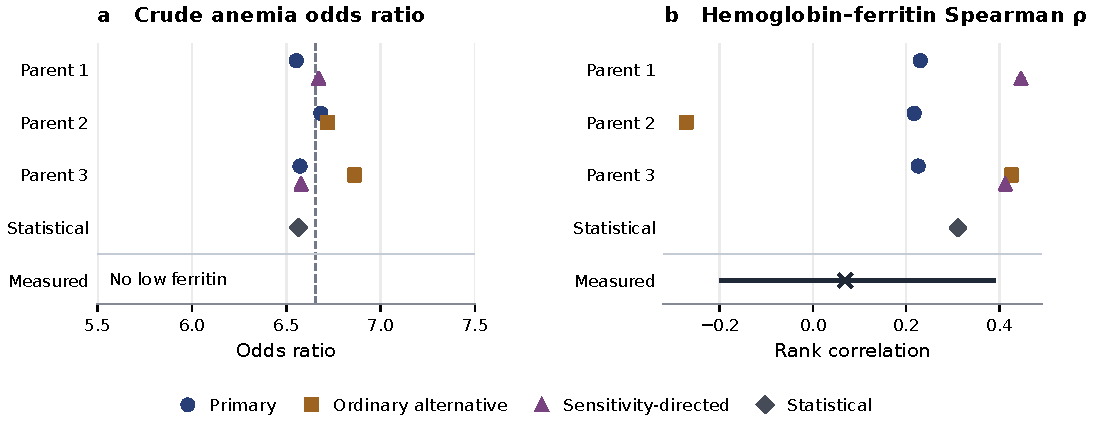
\includegraphics[width=.98\textwidth]{figures/iron-alternatives.pdf}
\caption{Two analyses on each sealed iron cohort. Symbols in each parent row distinguish the primary law and the two alternative requests. Two requests reached the output limit and have no point. The dashed line marks the source odds ratio of 6.65. The measured row gives the survey-weighted result for 44 women. The rank interval resamples villages within province. No woman in this sample had low measured ferritin.}
\Description{Agent odds ratios cluster between 6.55 and 6.86. Their rank correlations range from minus 0.272 to plus 0.446. The measured rank correlation is 0.069, with a wide interval.}
\label{fig:ironpros}
\end{figure*}

The protocol specified three independent primary sessions, two branches per primary, three seeds per executable law and 20,000 independent draws per seed. GPT-6.1 Sol received the original paper and a target description. It supplied the structure, parameters, prospective judgments and Python code. The statistical comparator used the same source and independent within-cell ranks. Two of nine requests (ordinary branch of parent 1, directed branch of parent 2) exhausted the 12,288-token output allowance. Usage across all nine requests cost an estimated US\$1.37 at the recorded tariff.

The original interface failed on all seven complete programs. Each program expected its named parameters at a different nesting level than the runner supplied. After the primary submissions were inspected and before simulated or measured outcomes were examined, we registered one mechanical rule to pass the nested parameter object following the same missing-key error on all three seeds. This rule preserved every scientific constant, line of sampler code, seed and target task. Original executions, failures and corrected executions were archived separately. The seven agent programs and one statistical program then produced 24 tables. All source assessments and model comparisons were committed before external disclosure.

The source checks cover four crude-cell frequencies, the crude log odds ratio, three hemoglobin-band frequencies, three ferritin-depletion fractions, three within-band ferritin geometric means, and both overall geometric means. These 16 checks overlap. Tolerances allow rounding, four estimated Monte Carlo standard errors and fixed operational allowances. Table~\ref{tab:ironprospective} gives the pooled simulated estimates. Each completed pair's absolute rank gap was 0.187--0.489. Subtracting its estimated 95\% Monte Carlo margin left 0.175--0.475. These margins describe simulation precision conditional on fixed laws.

\begin{table}[H]
\caption{Prospective iron analyses by parent and request. Each completed law contributes three draws. The last column records the complete source screen.}
\label{tab:ironprospective}
\centering
\begin{tabular}{@{}lrrl@{}}
\toprule
Construction & Odds ratio & Spearman $\rho$ & Screen\\
\midrule
P1 primary & 6.553 & 0.230 & pass\\
P1 ordinary & -- & -- & incomplete\\
P1 directed & 6.672 & 0.446 & pass\\
P2 primary & 6.683 & 0.217 & pass\\
P2 ordinary & 6.718 & -0.272 & pass\\
P2 directed & -- & -- & incomplete\\
P3 primary & 6.573 & 0.226 & pass\\
P3 ordinary & 6.862 & 0.426 & pass\\
P3 directed & 6.579 & 0.413 & pass\\
Statistical & 6.564 & 0.311 & pass\\
\bottomrule
\end{tabular}
\end{table}

\paragraph{What choices changed the continuous association?}
Three primary authors each received the article and the research request. Follow-up authors received a sealed primary program and either a request for another defensible model or for a sensitivity model. Four of the six requested pairs completed. In all four, the change in rank exceeded its simulation noise. Only one primary yielded both alternatives. For the second parent, the ordinary alternative used a Gaussian copula parameter of $-0.75$ within bands and changed rank correlation from $0.217$ to $-0.272$. This was an explicit assumption. For the third parent the two positive-dependence alternatives moved its rank from $0.226$ to $0.426$ and $0.413$. The Burkina Faso study provided 44 measured mothers from 23 villages~\cite{burkina_iron}. Eighteen had low hemoglobin, none had low ferritin, and both binary classifications agreed with the deposited flags for every woman.

\section{What can change while the selected iron summaries stay fixed?}
\label{app:ironproof}
Two iron-status experiments serve different purposes. Figure~\ref{fig:method} traces three programs written directly from the article. Figure~\ref{fig:ironworked} uses a separate set of seven programs that passed the source checks and illustrates why allocating continuous observations within the same threshold cell can change the rank association. The five drawn pairs are schematic. The two outcome panels use the actual seven programs.
\begin{figure*}[tbp]
\centering
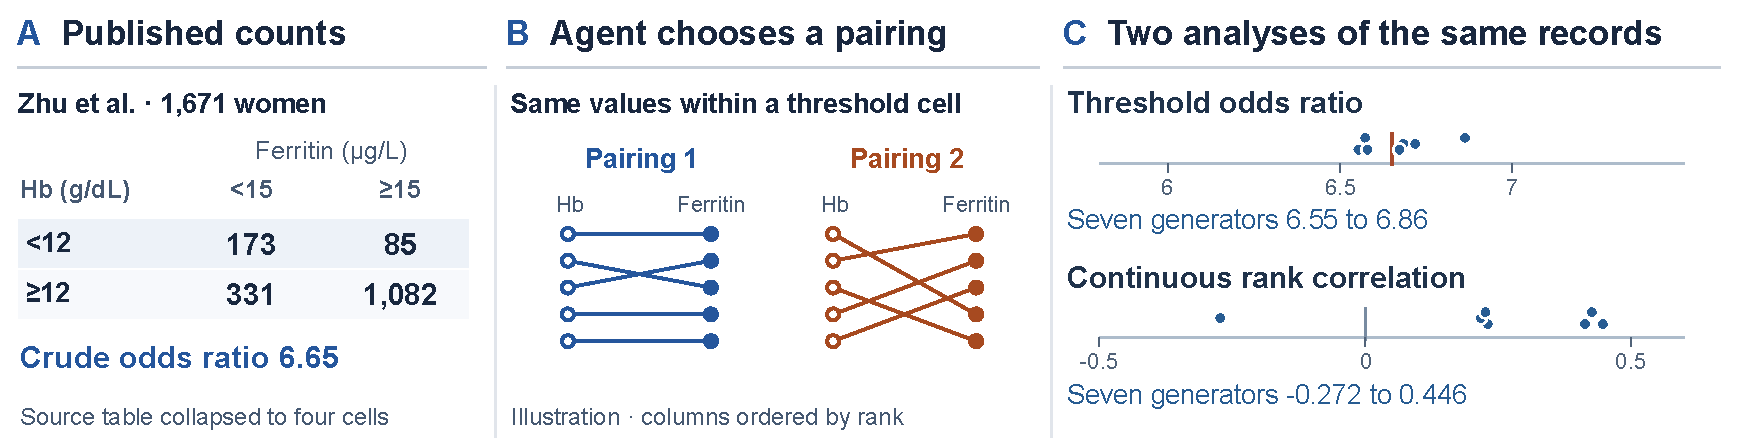
\includegraphics[width=\textwidth]{figures/evidence-and-pairing.pdf}
\caption{A worked example of evidence, model choice and downstream use. (A) Collapsing the iron-status groups in Zhu et al.~\cite{zhu} yields four counts and a crude anemia odds ratio (OR) of 6.65 for low versus higher ferritin. (B) The lines illustrate two ways of assigning the same five ferritin values to the same five hemoglobin values in one threshold cell. Either assignment preserves the cell count. (C) Seven programs that passed the source checks produced similar threshold ORs and a wide range of continuous Spearman correlations. Each dot is one program. The orange mark gives the source OR. The models see the reported band summaries as well as the counts.}
\Description{A two-by-two table implies an odds ratio of 6.65. Two illustrative matchings preserve the values assigned to the cell. Seven real program outputs give odds ratios from 6.55 to 6.86 and continuous correlations from minus 0.272 to 0.446.}

\label{fig:ironworked}
\end{figure*}


Take one cell of positive probability defined by hemoglobin band and ferritin depletion. Keep its probability and the two continuous conditional marginal distributions fixed. Draw hemoglobin from its conditional quantile function at a uniform rank $U$. One law draws ferritin from its conditional quantile at an independent uniform rank $V$. Another draws ferritin at $U$ with probability $\lambda>0$ and at $V$ otherwise. All other cells can stay fixed. The four threshold counts, each hemoglobin-band probability, and the ferritin geometric mean and depletion frequency in each band are invariant in the population. The overall geometric means are invariant as well.
For continuous marginal distributions, Spearman correlation is $12\,\mathbb{E}[F_H(H)F_F(F)]-3$. Within a nondegenerate cell the two marginal ranks are increasing functions of their corresponding uniforms. Sharing a uniform gives them positive covariance relative to independence. Hence the overall rank correlation changes while all the listed summaries remain fixed. This construction explains the ambiguity for the specified summaries. It supplies neither a biological estimate of the coupling nor its feasible range under additional evidence.

\section{Matched-size lifestyle analysis}
\label{app:lifestyle}
\begin{figure*}[t]
\centering
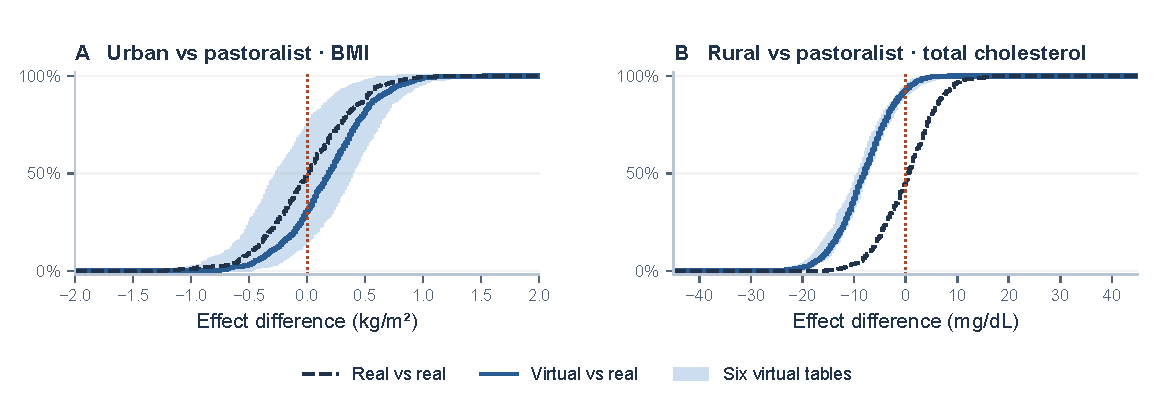
\includegraphics[width=.84\textwidth]{figures/lifestyle-main.pdf}
\caption{Signed differences across 500 matched resamples. Dashed curves compare two measured resamples. The blue line and band show the pointwise median and range of six virtual--real curves. The urban BMI discrepancies resemble real sampling variation. The virtual rural TC contrasts tend to be smaller.}
\Description{Cumulative curves overlap for the urban versus pastoralist BMI contrast. The virtual-versus-real curves shift left for rural versus pastoralist total cholesterol.}
\label{fig:lifestyle-sampling}
\end{figure*}


\begin{figure*}[t]
\centering
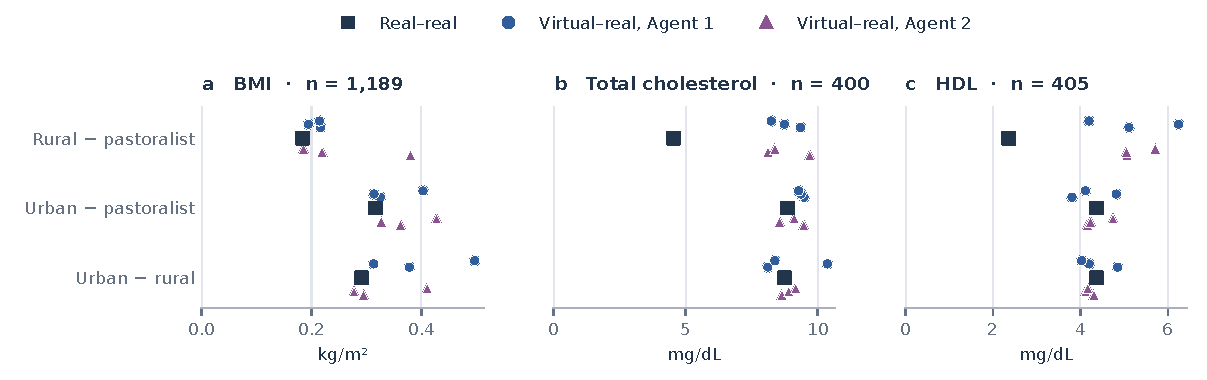
\includegraphics[width=.92\textwidth]{figures/lifestyle.pdf}
\caption{Matched-size mean absolute discrepancies for all nine adjusted lifestyle contrasts. The real--real estimate comes from two resamples of measured records. The virtual--real estimates use six saved virtual tables from two constructors. Native units and sample sizes differ across panels.}
\Description{Three panels compare BMI, total cholesterol and HDL across rural, urban and pastoralist lifestyles. Virtual versus real discrepancies are similar to real versus real for the urban BMI contrast, and larger for both rural lipid contrasts.}
\label{fig:lifestyle}
\end{figure*}

The original Turkana regression compared three lifestyle groups, adjusting each trait for age and sex~\cite{lea}. Real and virtual samples were matched on six sex-by-lifestyle stratum sizes within each trait. There were 1,189 eligible BMI measurements, 400 total cholesterol measurements and 405 HDL measurements. Each of 500 repetitions drew two real samples from the same empirical pool and one sample from each fixed virtual table. The virtual samples shared the second real sample as their reference. This design conditions on sample size, available cases and stratum counts. It leaves age and the outcomes free to vary. The bootstrap uses participants and does not model household or site clustering.



\begin{table*}[t]
\caption{Absolute discrepancies in matched-size lifestyle regressions. R and U denote rural and urban groups, and P denotes pastoralists. V--R gives the range across six fixed tables.}
\label{tab:lifestyle}
\centering
\begin{tabular}{@{}llrr@{}}
\toprule
Outcome & Contrast & Real--real & V--R\\
\midrule
BMI & R--P & .184 & .185--.380\\
(kg/m$^2$) & U--P & .316 & .314--.428\\
 & U--R & .291 & .277--.497\\
\midrule
Total cholesterol & R--P & 4.543 & 8.118--9.695\\
(mg/dL) & U--P & 8.848 & 8.556--9.479\\
 & U--R & 8.743 & 8.110--10.365\\
\midrule
HDL cholesterol & R--P & 2.363 & 4.195--6.242\\
(mg/dL) & U--P & 4.375 & 3.807--4.818\\
 & U--R & 4.362 & 4.029--4.851\\
\bottomrule
\end{tabular}
\end{table*}

Only 37 urban participants contributed total cholesterol measurements and 38 contributed HDL measurements. This small group helps explain the wide real--real variation. The discrepancy estimates in Table~\ref{tab:lifestyle} describe the observed composition. Equivalence for a planning decision would require a tolerance justified for that decision.

\section{Prospective external comparison in Akwa Ibom}
\label{app:akwa}
The Akwa Ibom study in southern Nigeria was second on the project's previously ordered list of iron cohorts. We screened the data dictionary, release terms, availability and uniqueness of participant keys before measuring either endpoint. Among the 1,290 biochemical records, 603 female participants in the mothers' group were aged 18--49 and had positive, finite Hb and serum ferritin. They came from 30 enumeration areas in 10 local government areas. The biochemical file supplies no analysis weight or pregnancy indicator. We report the sampled mothers' crude rank correlation and threshold odds using uncorrected ferritin. These characteristics limit transport from the Chinese cohorts. IITA and HarvestPlus supervised the original survey with support from the Bill \& Melinda Gates Foundation to HarvestPlus~\cite{akwa_iron}.

The article, aggregate supplement, task, seeds and hidden data digest were fixed before dispatch. The common virtual marginals came from the source-only CHNS A fit. Every law received the same sorted Hb and ferritin values in each of three Hb bands. The agent returned a sampler that assigns a permutation of ferritin values to the Hb values in each band, plus its parameters and their rationale. Six fresh sessions used the same GPT configuration. For the statistical arm we fit one Gaussian copula parameter to the supplied geometric-mean ferritin ratio of 1.215 comparing $13\leq\mathrm{Hb}<14$ with $12\leq\mathrm{Hb}<13$. Numerical integration gave a latent normal correlation of 0.137. The statistical law used this value in all three bands. Each law received the same three seeds and 12,000 virtual pairs per seed. Pairing preserves the threshold counts exactly across arms. The source ratio and each law's realized middle-band contrast remain available for checking.

We pooled each law's three draws for scoring and resampled whole enumeration areas within each local government area 2,000 times. Each paired bootstrap replicate compared all frozen laws with the same measured resample. Its interval describes sampling variation conditional on these particular constructors. The prespecified rule required at least four executable constructors, a median improvement of at least 0.02 in absolute rank error, a positive lower 95\% bound and a common threshold odds ratio within a factor of 1.50 of the measured odds ratio with at least ten observations per measured cell. Around a rank correlation of 0.30, the 0.02 margin corresponds to about a 13\% difference in an illustrative Fisher-transformation planning calculation.

\begin{table}[t]
\caption{Akwa Ibom external comparison. The middle-band ratio uses the two geometric mean ferritin levels defined above. The Chinese source ratio supplied to every constructor was 1.215.}
\label{tab:akwa}
\centering\small
\begin{tabular}{@{}lrrr@{}}
\toprule
Law or sample & Rank & Abs.\ rank error & Middle ratio\\
\midrule
Akwa Ibom sample & 0.0103 & --- & 0.9491\\
Statistical generator & 0.3031 & 0.2928 & 1.2254\\
Agent 1 & 0.3082 & 0.2979 & 1.2440\\
Agent 2 & 0.3082 & 0.2979 & 1.2440\\
Agent 3 & 0.3082 & 0.2979 & 1.2440\\
Agent 4 & 0.3082 & 0.2979 & 1.2439\\
Agent 5 & 0.3082 & 0.2979 & 1.2440\\
Agent 6 & 0.3082 & 0.2979 & 1.2440\\
\bottomrule
\end{tabular}
\end{table}

All six source programs and model responses had distinct hashes. At shared seeds five programs produced the same arrays, and the sixth produced slightly different arrays. The largest distance between any sealed agent rank and the statistical rank was 0.00509. By the reverse triangle inequality this also bounds the difference in their absolute errors for \emph{any} target rank. Consequently the 0.02 margin was already unattainable before disclosure. Both endpoints of the paired percentile interval rounded to $-0.00509$. Whenever the resampled reference rank falls below both estimates, it cancels from their paired error difference. The interval for the measured rank itself was much wider. This paired interval is conditional on the sealed laws and shared seeds. Table~\ref{tab:akwa} shows all constructions.

All four threshold cells in the measured sample contained at least 22 mothers. The common virtual odds ratio was 4.49 times the measured value, exceeding the 1.50 guard. The comparison preserves both virtual marginals in each band, so this discrepancy applies to both arms. Different source and target sampling frames, assays, inflammation and pregnancy status could influence transport. This experiment cannot assign the discrepancy to any one cause. The six calls cost an estimated US\$0.484 at the recorded tariff.

Independent scoring from the official Stata file reproduced the point estimates, the two measured intervals and the paired error interval. A check frozen before disclosure required identical ranks to $10^{-12}$ across the official Stata and text files. Text serialization merged the ranks of two ferritin readings. Its estimate differed by $4.32\times10^{-6}$, with the same threshold cells and decision. The separate code also checked all 21 virtual draws against their archived hashes and verified the two marginal multisets within every band.

\begin{figure*}[t]
\centering
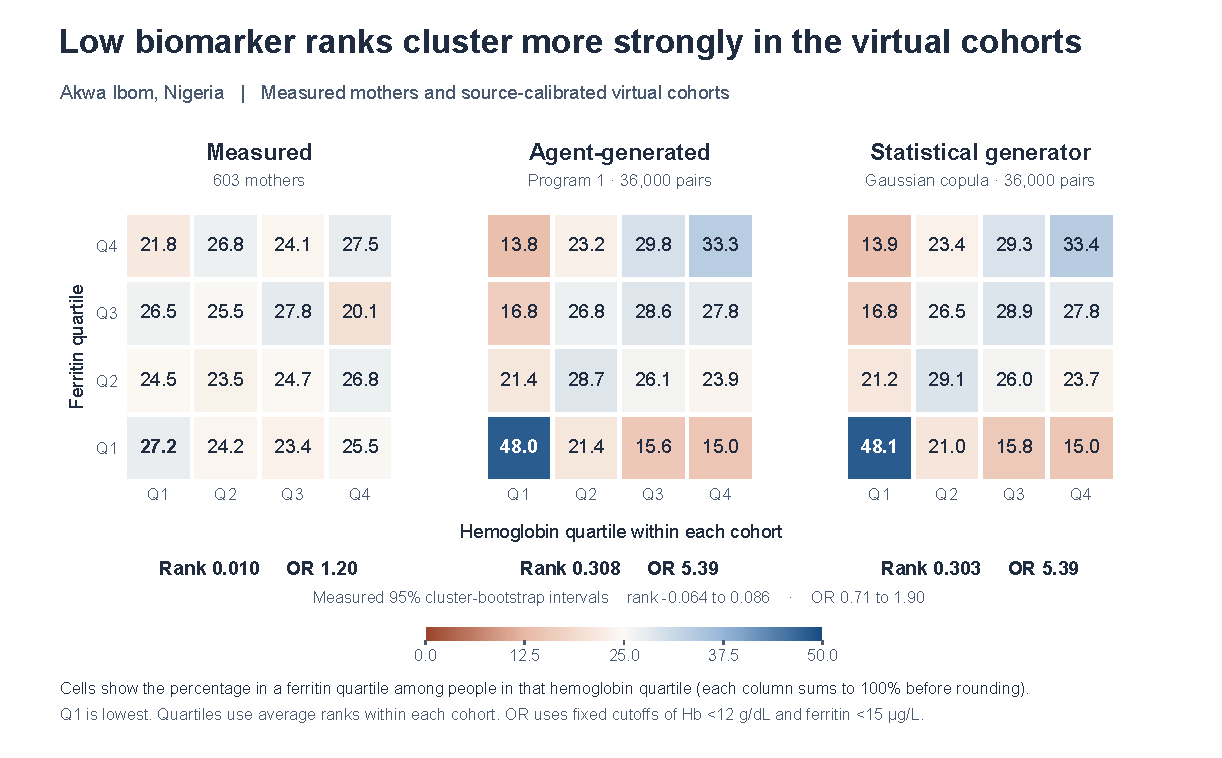
\includegraphics[width=.82\textwidth]{figures/akwa-heat.pdf}
\caption{Continuous ranks in Akwa Ibom, shown after outcome disclosure. Each cell gives the percentage in the specified ferritin quartile within a hemoglobin quartile. Quartiles are formed separately in the measured sample and each virtual law. The first prespecified agent is shown; all six have identical counts at this resolution. The odds ratios use absolute clinical cutoffs.}
\Description{Among mothers in the lowest hemoglobin quartile, the measured fraction also in the lowest ferritin quartile is 27.2 percent, compared with 48.0 and 48.1 percent in the virtual cohorts.}
\label{fig:akwa-heat}
\end{figure*}

\section{Audit of the two lipid comparisons}
\label{app:nonhdl}
The source sample was nonfasting. Mekelle used a Bio-system A25 and Haramaya a Mindray BS-200 on fasting samples. Neither cohort supplied measurements to either constructor. No reference rows were shared between the independently recruited study frames to our knowledge. The project used only the packet and no individual source records. The source mean ratio is the mean of individual ratios. For common lognormal margins, fitting the TC upper-cutoff probability allows two positive log SDs; we fixed the smaller one before generation. Each method used three seeds with 16,000 pairs per seed. Across the 48,000 records per method, HDL exceeded TC in 56 agent and 47 statistical pairs. The measured counts were zero in Mekelle and seven in Haramaya. All were retained as specified. These scientific outputs were computed after explicitly repairing the metadata interface; the raw automation had zero successful agent draws.

We resampled individuals 2,000 times within age groups 20--39 and 40 or older in each study. The 95\% intervals for the sample means were 120.19--130.00 and 120.96--126.27 mg/dL. The corresponding intervals for the fractions above or at the cutoff were 16.82--25.55\% and 18.64--23.20\%. Intervals condition on the observed age composition and frozen generators. They omit uncertainty in the original Tanzanian estimates and do not generalize the samples to the country. Among all possible permutations of the supplied empirical marginal arrays, 9.02--41.54\% can cross the threshold if no source ratio or physiological constraint is imposed. This is an outer diagnostic range for the source-constrained problem. It does not identify which assumption caused the external discrepancies.

\section{Auditing pairing decisions on frozen tables}
\label{app:pairingtest}
\paragraph{Lifestyle.} We examined all nine age- and sex-adjusted contrasts on each of the six existing tables. Conditional on the design matrix, an OLS contrast is linear in the outcomes. Under uniform joint permutation of the outcome vectors within each lifestyle-by-sex cell, its expected coefficient equals the coefficient obtained by substituting the cell means. We verified the expectation using centered within-cell covariances and exhaustive permutations on a small fixture. Real--real discrepancies are the archived mean absolute differences at matched sample size. The nine real effects were already known when this ablation was defined. The comparison measures how much this particular age pairing affected the estimate.

\paragraph{Lipids.} The protocol, source-only request, scorer, interface and budget were sealed before the four new calls. Each author received one call and had to supply a program with two scenarios. We then sealed all four programs before executing any. Each scenario used the same three ordered seeds and 16,000 observations per seed. Mean individual TC/HDL had to be within 0.02 of 3.66 on every seed and round to 3.66 in the pool. All clinical ordering constraints had to hold. Material sensitivity required a pooled difference exceeding four percentage points and a difference in the same direction exceeding two points on every seed. All four sessions met this criterion on the first call. Each marginal array had 14.4\% above the source TC cutoff and 15.3\% below the source HDL cutoff. The tariff estimate for four calls was US\$0.231. The observed seed spread measures simulation variability within a particular model pair.

\begin{figure*}[t]
\centering
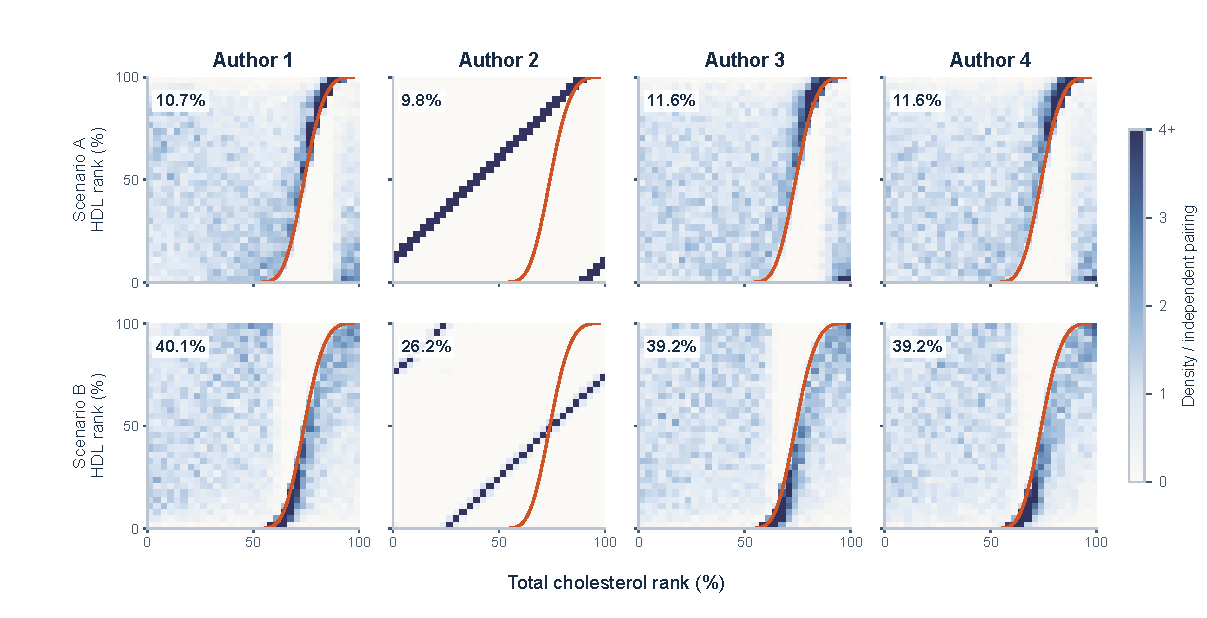
\includegraphics[width=.91\textwidth]{figures/lipid-rank-maps.pdf}
\caption{Two ways of assigning the same HDL measurements to the same total cholesterol measurements. The panels show all four authors on the first predeclared seed. Bin intensity is relative to independent rank pairing, on a common scale capped at four. Pairs below the orange curve have non-HDL at or above 160 mg/dL. Insets give the proportion from each complete draw. Author 2's rank cycles illustrate how a model can match the source ratio while imposing a distinctive joint structure.}
\Description{Eight rank density maps share the same axes. Orange curves mark the screening threshold. Opposite rank cycles are particularly visible for author two.}
\label{fig:lipidmaps}
\end{figure*}

The constructive control partitions the fixed order statistics into 125 interleaved blocks of 128. Linear assignment within each block supplies admissible permutations. Integer programming selects one per block while constraining the pooled ratio. Direct calculation on the full tables verified the two solutions. The 32.03-point spread is 98.5\% of the width of the unrestricted empirical bounds of 9.02--41.54\%. We establish two feasible points under the added conditions. The source summaries and the numerical test do not assign probabilities to the models in Figure~\ref{fig:lipidmaps}. Neither this separate four-author test nor the constructive control used another measured cohort.

\section{Prospective decisions on the Virginia sample}
\label{app:virginia}
\paragraph{Prospective decisions.}
\label{sec:virginia}
We kept the original virtual table fixed. Before opening a rural Virginia community screening study~\cite{virginiastudy,virginiadata}, eight fresh GPT sessions ranked six requested analyses. All saw the source summaries, virtual estimates, prior discrepancies in Ethiopia and a description of the new population. Four randomly assigned sessions also saw the numerical ranges from the eight agent-authored alternatives and two constructive examples. A statistical rule ranked uses by the largest available discrepancy or uncertainty relative to the intended tolerance. The rankings and unforced endorsements were sealed before we analyzed 400 adults.

\begin{figure*}[t]
\centering
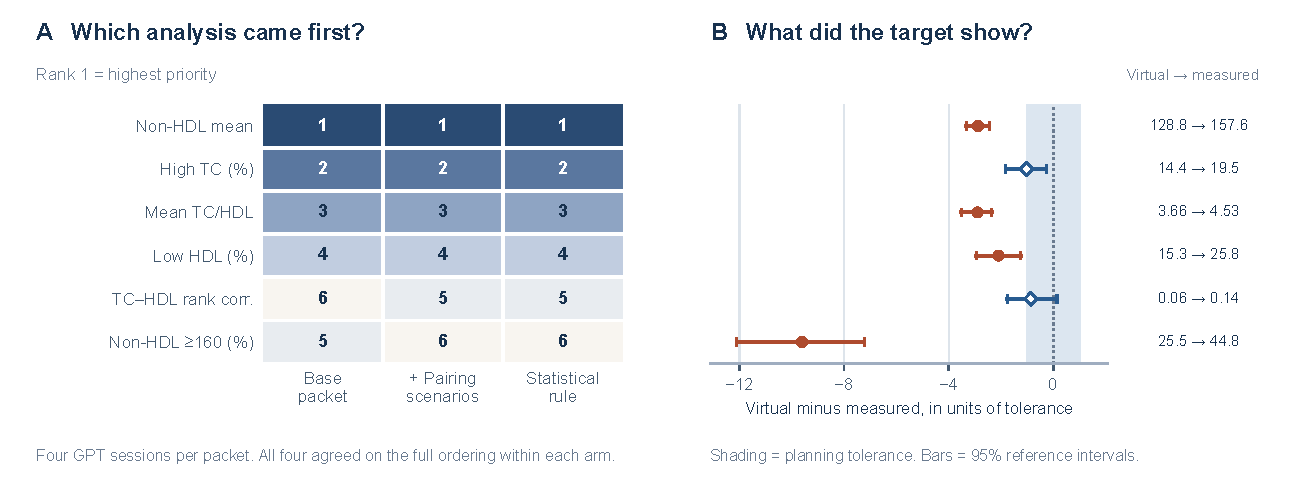
\includegraphics[width=.97\textwidth]{figures/decisions-before-disclosure.pdf}
\caption{Decisions made before access to the Virginia measurements. (A) The four advisers in each arm agreed on all six ranks. The rule received the full packet. (B) Values show the original virtual estimate and its measured counterpart. The scale is the signed difference divided by the use-specific planning tolerance. Bars are pointwise 95\% intervals from 4,000 within-county bootstrap resamples. A bar entirely within the shaded band would support that use at the declared tolerance.}
\Description{The two arms and the rule rank mean non-HDL and high TC prevalence first and second. Providing alternative pairings moves non-HDL screening from fifth to sixth. Its measured discrepancy is 9.61 tolerances. Four intervals lie outside the tolerance band and two overlap a boundary.}
\label{fig:decision}
\end{figure*}

At the primary coverage of two, all advisers and the rule chose mean non-HDL and high TC prevalence. The virtual mean was 128.77 versus 157.57 mg/dL measured, outside the $\pm10$ margin. The high-TC comparison was unresolved. Across all six uses, four intervals lay entirely outside their margins and two crossed a boundary. In the prespecified coverage curve, the arms differed only when selecting five uses. All four advisers shown alternatives set aside non-HDL screening, whose 25.53\% virtual estimate differed from 44.75\% measured by 9.61 tolerances. All four base-packet advisers set aside rank correlation instead. The statistical rule matched the full arm (Figure~\ref{fig:decision}). Seven advisers endorsed the mean when free to abstain. All eight declined to endorse the screening use.

A post-disclosure diagnostic identifies a concrete limit on revision. Across every pairing of the fixed source values the screening rate can reach at most 41.54\%. The observed Virginia rate exceeds this by 3.21 points, although its sampling interval overlaps the bound. Changing the pairing alone cannot close the observed gap at the stated two-point tolerance. The following analysis gives the margins and documents the missing second sampling frame.

\paragraph{Admission and information.}
Ten candidates were screened from study methods, participant-file documentation and prior exposure. The open Virginia study qualified for the community frame. The screened datasets for a separate type 2 diabetes frame lacked the paired biomarkers, documented subtype, individual release or independent provenance. The archive describes 403 screened participants among 1,046 rural African Americans interviewed~\cite{virginiadata,virginiastudy}. Eligibility required age at least 20, a known county and paired positive finite concentrations. The 400 eligible adults had distinct IDs, with 198 from Buckingham and 202 from Louisa. The archive's original S serialization reproduced the CSV on ID, county, age, both lipid values and the recorded ratio. All ratios for the analysis were calculated from the two component measurements. The agent saw an anonymous study description. Prior model exposure to this widely used dataset is possible. Individual fasting, assay and treatment details could not be standardized across studies.

\paragraph{Decisions and scoring.}
The full packet adds the numerical ranges of ten source-compatible alternatives to the base packet. Four randomly assigned sessions per arm used GPT-6.1 Sol at medium effort. The eight one-call response tariffs totaled US\$0.06262. The statistical rule takes the largest of three available displacements: the more distant source confidence limit from the reported point, the largest historical measured discrepancy from the fixed virtual estimate, and the largest shift under any alternative model. It scales each by the use's planning margin. Lower scores receive higher priority. A score of at most one receives an endorsement. All nine decision records were sealed before the six measured estimates were opened. We formed pointwise percentile intervals using 4,000 participant bootstrap draws stratified by county with its sample size fixed, recomputing tied ranks in each draw. Intervals compare the measured estimate to the fixed virtual table under the specified sampling assumptions.

The six margins in their original units are 10 mg/dL for mean non-HDL, 0.30 for mean individual TC/HDL, five percentage points each for high TC and low HDL, two points for non-HDL at least 160 mg/dL and 0.10 for Spearman correlation. The high-TC and low-HDL cutoffs were 6.2 and 1.0 mmol/L with respective inclusive upper-tail and strict lower-tail rules. At the original tolerance, none of the six measured intervals fit wholly within its margin. At twice the margin, the high-TC prevalence and rank correlation did. All six coverage levels and three tolerance scales were registered. The five-use illustration was selected for discussion after disclosure. The mean absolute discrepancy among those five uses was 3.70 times tolerance with the base packet and 1.95 times with alternatives. Both retained sets contained zero fully supported analyses. The two county subsets are secondary checks within one study.

\begin{figure*}[t]
\centering
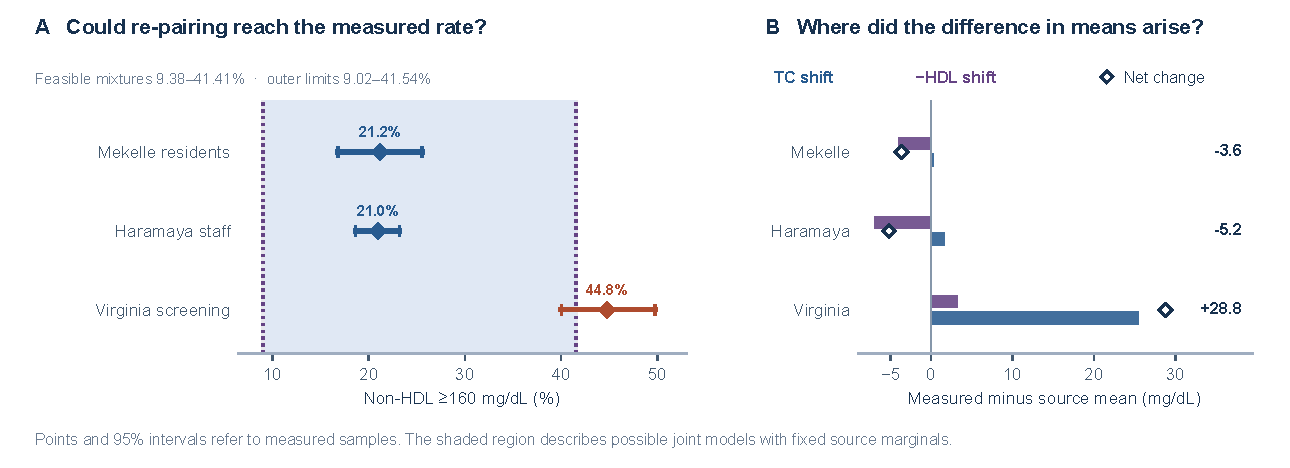
\includegraphics[width=.96\textwidth]{figures/where-pairing-can-help.pdf}
\caption{What could changing the lipid pairing correct? (A) The shaded interval contains all intermediate population-level screening fractions attainable by random mixtures of two source-compatible joint laws. Dashed lines mark the extremes over arbitrary pairings of these fixed marginal values. Measured points and intervals are shown for the two historical Ethiopian cohorts and the new Virginia study. (B) Mean non-HDL is linear in the component means. Each diamond marks the signed sum of the TC shift and the contribution of the HDL shift.}
\Description{Both Ethiopian point estimates and their intervals lie inside the achievable range. The Virginia point estimate lies outside the unrestricted upper bound while its interval overlaps. Its positive mean difference comes mostly from higher TC.}
\label{fig:repair}
\end{figure*}

\paragraph{A retrospective diagnostic for choosing the next measurement.}
For fixed empirical TC and HDL marginals, a mixture of two joint laws retains those marginals. Both the expected individual ratio and threshold probability are linear in the mixing weight. The two admissible numerical examples attain 9.375\% and 41.40625\% screening. Random mixtures attain every intermediate population-level probability and retain the accepted mean-ratio interval and component ordering. An independent count of feasible threshold matches, including ties, reproduced the unrestricted empirical limits of 9.01875\% and 41.54375\%. The resulting feasible interval spans 98.48\% of the outer width. These constructed laws carry no likelihood weights. The diagnostic was planned after the Virginia discrepancy was observed. In Ethiopia all four agent-authored scenario pairs bracketed both measured rates. In Virginia 179/400 participants crossed the threshold (44.75\%, 95\% interval 39.99--49.75\%). Its sampling interval intersects the feasible region (Figure~\ref{fig:repair}A). The 28.79 mg/dL change in mean non-HDL equals the sum of a 25.52 mg/dL rise in mean TC and a 3.28 mg/dL contribution from lower HDL, before rounding (B). Even complete knowledge of the ordering could not change that mean.

\begin{table*}[t]
\centering
\caption{Six prespecified analyses on the original lipid pairing and the same people after both historical means were adopted. Percentages and their tolerances are in percentage points. Parentheses give survey-design 95\% intervals. A use is supported when the entire interval is within its stated margin of the virtual estimate.}
\label{tab:historicalmeans}
\small
\begin{tabular}{lrrrrr}
\toprule
Analysis & Margin & Original & Updated & US 2017--2018 & US 2021--2023 \\
\midrule
Mean non-HDL (mg/dL) & 10 & 128.77 & 143.50 & 135.47 (131.87--139.06) & 135.02 (132.71--137.33)\\
Mean individual TC/HDL & 0.30 & 3.659 & 4.023 & 3.790 (3.690--3.890) & 3.732 (3.661--3.802)\\
High TC (\%) & 5 & 14.40 & 20.50 & 10.52 (8.89--12.15) & 11.21 (9.75--12.68)\\
Low HDL (\%) & 5 & 15.30 & 17.35 & 13.86 (11.53--16.20) & 11.92 (10.14--13.69)\\
Non-HDL $\geq160$ mg/dL (\%) & 2 & 25.53 & 34.25 & 25.33 (22.59--28.07) & 24.25 (22.40--26.09)\\
TC--HDL Spearman correlation & 0.10 & 0.059 & 0.059 & 0.137 (0.086--0.187) & 0.206 (0.176--0.236)\\
\bottomrule
\end{tabular}
\end{table*}

\section{Historical US information and two later survey periods}
\label{app:historicalmeans}
\begin{figure*}[t]
\centering
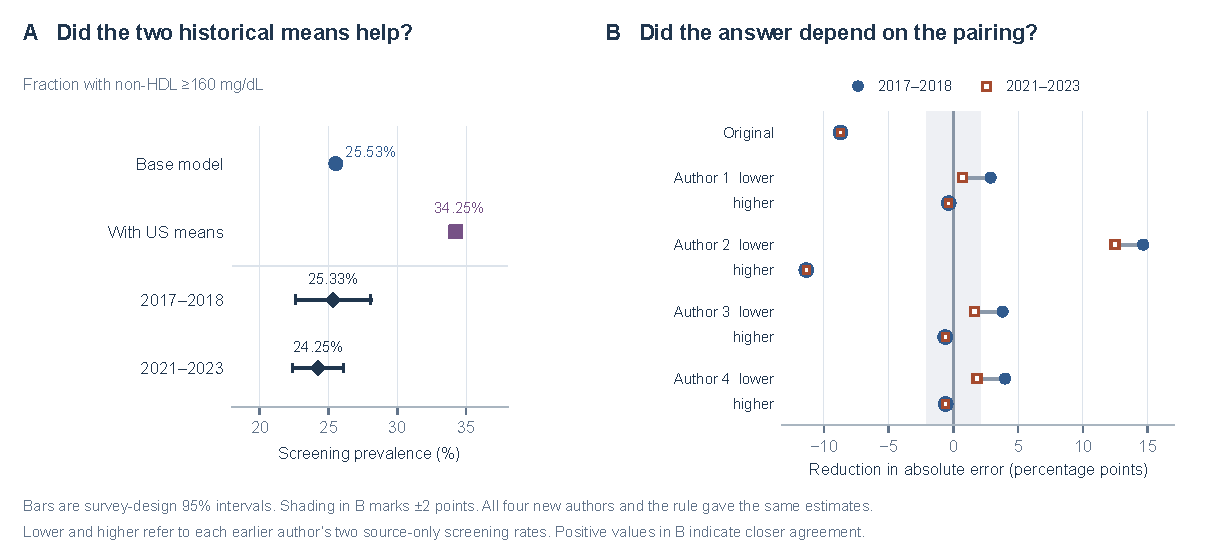
\includegraphics[width=.96\textwidth]{figures/historical-means-and-pairing.pdf}
\caption{Adding the same two historical US means to nine frozen lipid pairings. (A) On the original pairing the update raises the predicted screening rate above both later national estimates. (B) Each point shows the reduction in absolute error for one period and pairing. Positive values mean closer to the survey estimate. The line connects the two periods for a given pairing. Only panel A displays survey intervals. The four pairs of alternatives had been authored in a previous experiment.}
\Description{The original prediction goes from 25.53 to 34.25 percent. Both measured estimates are below 26 percent. For each of four authors, on both survey dates the alternative with the lower initial screening rate benefits at the survey point while the higher one deteriorates. Only one lower alternative benefits across both entire intervals.}
\label{fig:historicalmeans}
\end{figure*}

Mwanza reported the mean of the ratios formed within individuals (3.66) alongside the separate marker means and frequencies~\cite{kavishe}. Our historical US inputs were the 2007--2010 entries in Table~1 of Carroll et al.~\cite{carroll_history}, for adults aged 20 or older of both sexes (11,028 participants). The reported age-standardized 95\% intervals were 195--198 mg/dL for TC and 51.8--53.2 for HDL. These inputs contain no target-period joint threshold or mean individual ratio. The four authors, the proportional rule and the original model were evaluated under all nine frozen pairings. The three seeds within each pairing approximate its sampling law. All new authors used the same model and chose the same numerical transformation. Independent parsing, scoring and seed-level checks reproduced all 54 method-by-pairing combinations.

The US comparison retained adults aged 20 or older with both markers, including those taking lipid-lowering medication. We used the examination weight for 2017--2018 and the phlebotomy weight for August 2021--August 2023~\cite{cdc_lipids_l}. We directly standardized to the US year-2000 adult age distribution (20--39, 40--59 and 60+). Each of 15 masked strata contributed two primary sampling units per wave. We restandardized after each stratified delete-one-unit jackknife replicate and formed two-sided intervals using 15 degrees of freedom. The intervals quantify measured-sample variation conditional on the sealed virtual predictions. Both periods are later waves of the same survey family as the historical source.



The primary decision required a reduction of at least two percentage points in median author absolute screening error in both periods on the original pairing. Before disclosure, the screening rate at which the original and updated predictions would be equally close was 29.89\%. Both measured intervals fell below this point. Over these intervals the gain ranged from $-8.72$ to $-3.63$ and from $-8.72$ to $-7.59$ points respectively. Although the original screening predictions were close to both measured points, their intervals crossed the two-point use margin. Table~\ref{tab:historicalmeans} reports the five secondary analyses on exactly the same records. The high-TC and low-HDL cutoffs were $\geq6.2$ and $<1.0$ mmol/L respectively.

\paragraph{Which virtual participants crossed the threshold?}
Each update multiplied TC by $a=1.07384$ and HDL by $b=0.97672$. A participant previously below 160 mg/dL crossed exactly when the original TC lay in $[(160+b\,\mathrm{HDL})/a,\,160+\mathrm{HDL})$. A separate count reproduced every change in prevalence at each seed. From 0.36\% to 26.34\% of virtual participants crossed under the eight alternatives. All eight were prespecified. Grouping the alternatives by their original screening rate and tracing individual crossings were retrospective explanations. Across both entire survey intervals, one of the four initially lower scenarios improved and all four initially higher scenarios worsened. The arithmetical consequences differ by analysis. The mean individual ratio is multiplied by $a/b$ (a 9.94\% rise), the rank correlation is invariant, and the updated mean non-HDL is the difference between the two historical means. The four methods' common choice to preserve shape leaves other marginal transformations unevaluated.

\section{Bilateral grip and three recruitment settings}
\label{app:grip}

\begin{figure*}[t]
\centering
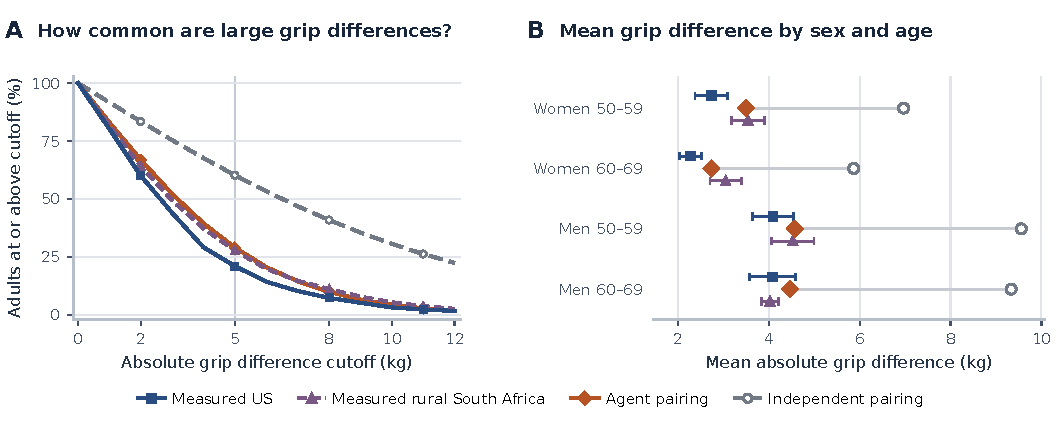
\includegraphics[width=.98\textwidth]{figures/grip-use-by-group.pdf}
\caption{Two uses of the same frozen handgrip data. (A) Each curve gives the percentage of adults whose two hands differ by at least the indicated amount, standardized equally across four sex-by-age groups. The vertical guide marks the previously specified 5 kg cutoff. (B) Within each group, the diamond and open circle use identical single-hand values. The two measured estimates have pointwise 95\% sampling intervals. The threshold sweep and subgroup comparisons were calculated after the original two population results were known.}
\Description{At the 5 kg cutoff, independent pairing gives 60.2 percent and the agent gives 28.9 percent, compared with 21.0 percent in the US and 27.7 percent in rural South Africa. In all eight subgroup comparisons the agent's mean gap is closer to the measured point than independent pairing.}
\label{fig:gripgroups}
\end{figure*}
\begin{figure*}[t]
\centering
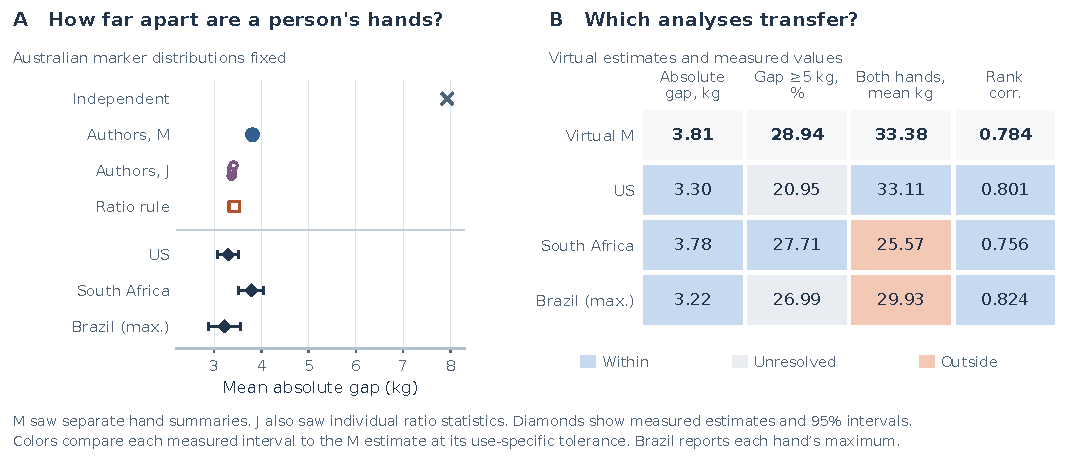
\includegraphics[width=.97\textwidth]{figures/bilateral-grip-transfer.pdf}
\caption{Pairing identical single-hand values changes the estimated difference between a person's hands. M authors saw separate Australian hand summaries. J authors also saw the dispersion of individual ratios in a German study. (A) Measured intervals cover sampling variation in each reference. (B) The same M table supports different analyses in different populations. The Brazil release uses each hand's maximum across attempts.}
\Description{Independent pairing gives a mean gap of 7.93 kg. The four M authors' common pairing gives 3.81, against 3.30 in the US and 3.78 in South Africa. A matrix compares four uses with complete sampling intervals. The South African and Brazilian bilateral means fall outside tolerance.}
\label{fig:grip}
\end{figure*}

\paragraph{Information and scientific uses.}
Massy-Westropp et al.~\cite{grip_adelaide} published anatomical right and left means and SDs in four strata (men and women aged 50--59 and 60--69). Their seated protocol averages three Jamar trials and excludes participants with hand pain or arthritis. We gave each stratum equal weight, constructed positive normal quantile grids rescaled to its two means and SDs, and fixed all 4,096 values for each hand in each cell. Four marginal-only (M) and four joint-evidence (J) sessions used the same GPT-6.1 Sol configuration. J also received the mean (0.9534) and SD (0.1100) of individual nondominant-to-dominant ratios from Wunderle et al.~\cite{grip_ratio}. That study pooled 444 non-left-handed adults across ages and sexes, using a pressure device. The instrument, definition of hand, and population all differ from the Australian report.

\begin{table*}[t]
\caption{Four scientific uses of the same handgrip records. Square brackets give pointwise 95\% measured-sample intervals. A virtual range covers the four J authors; all four M authors produced a single assignment for each seed. The planning margins were 1 kg, 5 percentage points, 2 kg and 0.10, respectively.}
\label{tab:grip}
\centering\small
\begin{tabular}{lrrrr}\toprule
Setting or construction & Mean absolute gap (kg) & Gap $\geq$5 kg (\%) & Mean of both hands (kg) & Rank correlation\\\midrule
US NHANES ($n=1{,}423$) & 3.30 [3.07, 3.52] & 20.95 [17.49, 24.40] & 33.11 [32.26, 33.96] & .801 [.751, .851]\\
South Africa HAALSI ($n=2{,}434$) & 3.78 [3.52, 4.05] & 27.71 [25.00, 30.42] & 25.57 [25.01, 26.12] & .756 [.718, .794]\\
Rio Branco maximum ($n=464$) & 3.22 [2.89, 3.55] & 26.99 [21.99, 32.00] & 29.93 [29.04, 30.82] & .824 [.783, .865]\\\midrule
M authors & 3.814 & 28.94 & 33.375 & .784\\
J authors & 3.371--3.413 & 23.40--23.53 & 33.375 & .837--.839\\
Ratio-based statistical model & 3.424 & 23.75 & 33.375 & .836\\
Independent pairing (expectation) & 7.932 & 60.24 & 33.375 & .000\\\bottomrule
\end{tabular}
\end{table*}

\begin{table*}[t]
\caption{Mean absolute between-hand grip difference in kg. Marginal-only authors all returned the same pairing. J authors also received the German hand-ratio evidence. Each measured interval is pointwise. Each method uses the same Australian single-hand values.}
\label{tab:gripgroups}
\small\centering
\begin{tabular}{@{}llrrrrrr@{}}
\toprule
Study & Sex and age & $n$ & Measured [95\% interval] & Independent & Agent, marginals & Agent, J range & J rule\\
\midrule
US NHANES & Women 50--59 & 378 & 2.73 [2.37, 3.09] & 6.97 & 3.50 & 3.00--3.15 & 3.03\\
 & Women 60--69 & 332 & 2.28 [2.03, 2.52] & 5.87 & 2.73 & 2.32--2.40 & 2.31\\
 & Men 50--59 & 362 & 4.09 [3.64, 4.55] & 9.56 & 4.57 & 4.02--4.36 & 4.39\\
 & Men 60--69 & 351 & 4.08 [3.58, 4.58] & 9.34 & 4.47 & 3.94--3.97 & 3.97\\
\addlinespace
Rural South Africa & Women 50--59 & 710 & 3.54 [3.18, 3.90] & 6.97 & 3.50 & 3.00--3.15 & 3.03\\
 & Women 60--69 & 597 & 3.05 [2.70, 3.39] & 5.87 & 2.73 & 2.32--2.40 & 2.31\\
 & Men 50--59 & 544 & 4.52 [4.05, 4.99] & 9.56 & 4.57 & 4.02--4.36 & 4.39\\
 & Men 60--69 & 583 & 4.02 [3.84, 4.21] & 9.34 & 4.47 & 3.94--3.97 & 3.97\\
\addlinespace
Rio Branco (max.) & Women 50--59 & 82 & 2.53 [2.09, 2.97] & 6.97 & 3.50 & 3.00--3.15 & 3.03\\
 & Women 60--69 & 195 & 2.43 [2.10, 2.77] & 5.87 & 2.73 & 2.32--2.40 & 2.31\\
 & Men 50--59 & 44 & 4.44 [3.54, 5.34] & 9.56 & 4.57 & 4.02--4.36 & 4.39\\
 & Men 60--69 & 143 & 3.47 [2.69, 4.26] & 9.34 & 4.47 & 3.94--3.97 & 3.97\\
\bottomrule
\end{tabular}
\end{table*}


\paragraph{Prospective paired measurements.}
The US NHANES 2011--2012 examination~\cite{grip_cdc} gives randomized starting hand, bilateral trials and effort flags. We required maximal effort on the first two trials for each hand and a positive examination weight. HAALSI baseline v3~\cite{grip_haalsi} supplied two cleaned measurements for each anatomical hand in rural Agincourt. We used the within-hand trial mean in both main settings. The separate Rio Branco study~\cite{grip_rio} released only the maximum per hand. We required both upper limbs to be eligible in that dataset. All settings weighted the four sex-by-decade cells equally. Within cells we used the US examination weights, Rio survey weights and equal weights in Agincourt. Pointwise intervals use a delete-one-cluster jackknife and $t$ quantiles with 17, 26 and 78 design degrees of freedom in the US, South Africa and Brazil. Rank correlation is the equally weighted average of within-cell weighted Spearman correlations. The Brazilian study was designated as a measurement stress test before scoring. The investigator had seen ancillary single-hand descriptions during admission. Both main survey families had appeared in other analyses. Constructors received no target participant measurements, single-hand summaries or paired estimates.

\paragraph{What did the additional evidence change?}
Three J programs derived dependence from ratio dispersion; one used 0.85 as a working correlation. The statistical rule estimated a within-cell correlation from the marginal coefficients of variation and the variance of log ratio, then paired ranks with a Gaussian copula. This rule shares J's indirect analogy between a pooled German pressure ratio and anatomical force ratios. The four independent M sessions returned distinct code but identical assignments for every shared seed. J returned four distinct assignments. Each of the eight programs generated 16,384 records at each of three seeds. The recorded tariff estimate for the eight completions was US\$0.2622.

Table~\ref{tab:grip} reports all observed uses. The US and South African point gains of 4.12 kg relative to independent pairing coincide because both measured mean gaps fall below both predictions. Holding the virtual outputs fixed, the mean-gap improvement from M to the median J author ranged from $+0.16$ to $+0.43$ kg across the US reference interval, and from $-0.43$ to $+0.16$ kg across South Africa's. At their respective measured points the gains were $+0.43$ and $-0.37$ kg. In Brazil the point gain was $+0.43$ kg. The same-evidence statistical rule was within 0.05 kg of the median J absolute error at every measured point.

\paragraph{Mean gaps inside the standardization groups.}
We reopened the three measured samples after the pooled results were known, used the archived eligibility rules and survey designs, and analyzed each sex-by-decade group. Source marginal grids, accepted permutations and sampling seeds were fixed. All eight point discrepancies in the two primary settings were within 1 kg. Seven measured intervals lay entirely within 1 kg of the corresponding fixed agent estimate. The US women aged 50--59 had a measured mean of 2.73 kg (2.37--3.09) against 3.50 kg generated. These are descriptive applications of the pooled study's 1 kg margin. The pointwise intervals account for participants' sampling structure and the four cells share one study design. Table~\ref{tab:gripgroups} includes all three populations. The Brazilian comparisons use maximal trials. No cell was used to select or revise a model.

\paragraph{What else could the source have supported?}
Holding the finite Australian grids fixed, pairing the order statistics in the same or reversed order gives the exact minimum and maximum possible mean gaps, 1.75 and 11.12 kg. This follows from the two-pair exchange inequality for absolute distance. In a retrospective continuous Gaussian calculation, common within-cell correlations from 0.762 to 0.883 place the virtual estimate within 1 kg over both complete principal reference intervals (Figure~\ref{fig:gripsens}). No new author, participant draw or coefficient fit enters this calculation. A separate prespecified diagnostic replaced the Australian marginals with each target's two separate empirical quantile grids and kept the archived permutations. M's mean gaps became 3.60, 3.97 and 3.97 kg in the US, South Africa and Brazil. The bilateral means then agreed within 0.002 kg by construction. This same-sample diagnostic illustrates how improving the overall marker levels can leave the between-hand discrepancy larger.

\begin{figure}[t]
\centering
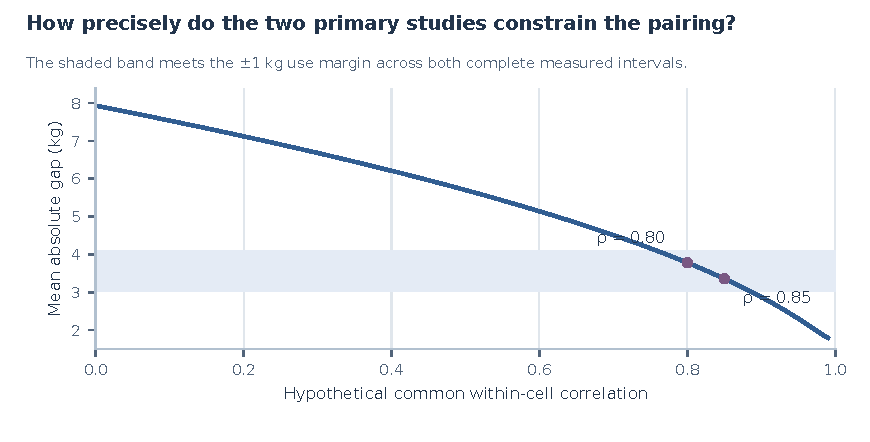
\includegraphics[width=.99\columnwidth]{figures/grip-correlation-sensitivity.pdf}
\caption{Retrospective sensitivity of the expected gap to a common within-group correlation under continuous normal single-hand distributions. The shaded band includes virtual gap estimates within 1 kg over both primary measured intervals.}
\Description{A curve slopes down from 7.93 kg at zero correlation to 1.75 kg near perfect correlation. The virtual mean gap is inside the shaded band for correlations of approximately 0.762 to 0.883.}
\label{fig:gripsens}
\end{figure}

\section{Prospective test of source evidence for spirometry}
\label{app:spirometry}
\begin{figure*}[t]
\centering
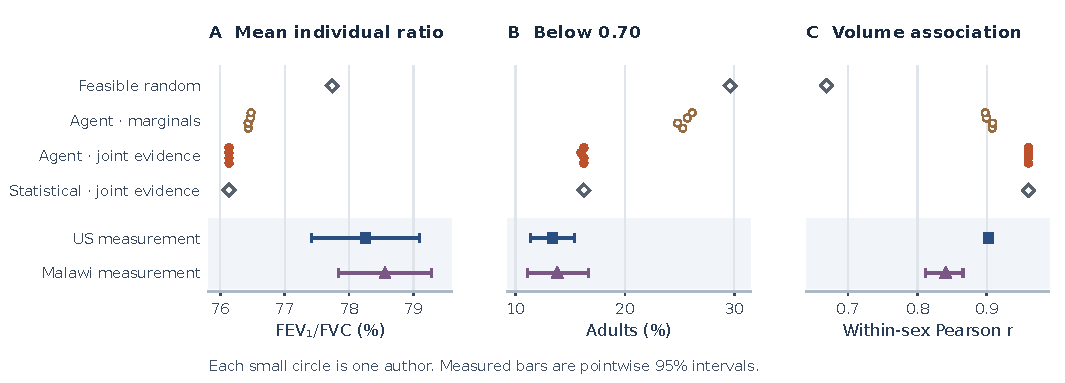
\includegraphics[width=.985\textwidth]{figures/spirometry-uses.pdf}
\caption{Three prespecified scientific uses of the same frozen virtual lung-function records. Small circles denote individual authors averaged over three draws. Diamonds denote the statistical rules. Measurements are sex-standardized with pointwise 95\% intervals. Full joint evidence moves the estimated fraction below 0.70 toward both samples while moving the within-sex correlation farther away.}
\Description{Four authors per evidence condition pair the same two volume columns. Adding joint evidence changes median predictions from 76.45 to 76.14 percent on the mean individual ratio, from 25.50 to 16.26 percent on the fraction below 0.70, and from 0.904 to 0.960 on correlation. The statistical rule given the same joint evidence nearly coincides with the full-evidence authors.}
\label{fig:spirometry}
\end{figure*}
The request concerned pre-bronchodilator FEV$_1$ and FVC in adults aged 18--79. We estimated the mean of individual ratios, the ratio of group means, the fraction with individual ratio below 0.70, and the average of the two within-sex Pearson correlations. All four uses give the sexes equal weight. The low-ratio fraction describes the research sample. Clinical diagnosis was outside its scope.

\paragraph{Which decision did the authors make?}
The Polish source examined 1,120 men and 1,625 women aged 18--85 who were healthy and had never smoked~\cite{polishspi}. Four independent GPT sessions received the sex-specific arithmetic means and SDs of both measurements. Four other sessions received those summaries and the within-sex Pearson correlations and regressions from the same study. Every session wrote its own pairing program for the same fixed volume columns. The four marginal-only authors each chose a working latent correlation of 0.90. The four full-evidence authors selected Gaussian rank models consistent with the published correlation of 0.96. A separate statistical generator fitted the latent correlation under a bivariate lognormal model. A second control sampled uniformly among feasible pairings. All final source-only pairs satisfied FEV$_1\leq{}$FVC. Individual ratios and the fraction below the cutoff can change with pairing. The ratio of the two means stays fixed.


\paragraph{Independent measured references.}
All predictions were sealed before the two samples were scored. The US survey supplied 3,945 adults with a completed baseline exam and grades A or B for both volumes. Intervals use examination weights and a stratified delete-one-PSU jackknife~\cite{cdcspiro}. In rural Malawi, the first public pre-bronchodilator pairs are from the first follow-up. Of 628 returnees, 586 qualified~\cite{malawispi}. We bootstrapped people within sex 2,000 times. Village identifiers and design weights were unavailable. We retained three quality-eligible measured pairs with FEV$_1$ above FVC. The Polish study recruited healthy never-smokers.

\paragraph{Planning margins and measured discrepancies.}
Adding the joint block reduced the median author's absolute error in the fraction below 0.70 by 9.24 percentage points at each measured point. Both target estimates lie below both median predictions, so this contrast has the same size by arithmetic. All four full-evidence programs stayed within the five-point planning margin throughout the US interval. One did so throughout the Malawi interval and the other three crossed its boundary. For the primary mean individual ratio, adding the block increased median absolute error by 0.32 points in both samples. The full-evidence prediction of 76.14\% compares with 78.26\% measured in the US and 78.56\% in Malawi.

\newpage
For the ratio of group means, all pairings gave 76.32\%, against 78.34\% and 78.44\%, respectively. Both ratio uses had a two-point planning margin. For the within-sex correlation, all full-evidence predictions exceeded the 0.05 tolerance throughout both measured intervals (Figure~\ref{fig:spirometry}).

\paragraph{How much could the agent improve on the statistical rule?}
Let $s$ be a statistical prediction, $a_i$ the prediction from author $i$, and $y$ a measured reference. By the reverse triangle inequality, the difference between $|s-y|$ and $|a_i-y|$ lies between $-|a_i-s|$ and $|a_i-s|$. Taking medians gives the bound $\bigl||s-y|-\mathrm{median}_i|a_i-y|\bigr|\leq\mathrm{median}_i|a_i-s|$. The frozen predictions bounded the median error difference at 0.000101 percentage points for the mean ratio and 0.00407 for the low-ratio fraction. The primary one-point gain was therefore out of reach at either site before disclosure. This bound compares methods. Absolute accuracy still depends on the measured reference.

\paragraph{Marginal distributions after disclosure.}
As a diagnostic we supplied each sample's measured marginal distributions and kept its source-based pairings fixed. The full-evidence median mean individual ratio moved toward the measured value, to 78.02\% in the US and 78.25\% in Malawi. The estimated fraction below 0.70 moved farther away, to 8.93\% and 7.15\%. Independent code reproduced all four uses on the 30 virtual tables and both measured samples. Exact decimal arithmetic confirmed every cutoff classification.
\clearpage

\section{Registered construction and analysis in the three matched articles}
\label{app:matchedprotocol}
The source and analytic request were held fixed within each article. The targeted and ordinary follow-ups used separate contexts with identical initial submissions. The agent supplied its evidence extraction, a model specification, Python sampler and decision record. The host constructed the single-marker grids from the extracted inputs, verified the scientific constraints, and used three registered seeds per program. Both branches were withheld after one incomplete lung submission. The 36 assigned initial blocks produced 106 actual calls, 105 eligible programs and 315 independently recalculated tables. All twelve assigned blocks per article entered each arm's denominator. The usage-derived total was US\$7.43. The registered expansion stopped after the iron arms tied. The measured handgrip experiment reported in the main text was a separate prospective study.

For lipids the target use was the fraction with non-HDL at least 160~mg/dL, while the companion was mean non-HDL. The change had to exceed four percentage points pooled and two at every seed in the pooled direction. For lung function the corresponding limits were five and two points for the fraction with individual FEV$_1$/FVC below 0.70. The mean-volume ratio was 76.24\% using the registered unrounded values. A common rounding convention made the source means and SDs jointly compatible with the sex-specific regressions and correlations at their printed precision. The iron thresholds were 0.10 pooled and 0.05 per seed for Spearman correlation. Authors retained the original band sizes, four joint counts, depletion proportions and geometric means at their printed precision. The crude odds ratio 6.653 and the separately reported adjusted odds ratio 6.448 are distinct estimands. Tolerances quantify sensitivity for the declared research use.

The three per-article exact tests used the discordant matched blocks. The ordinary-only and targeted-only counts were 0 and 11, 0 and 5, and 0 and 0. The corresponding two-sided \(p\)-values are 0.00098, 0.0625 and 1 under the registered rule for a tie. The article-level comparisons were sequential. They do not estimate a probability of success over a random sample of biomedical publications.

\paragraph{Numerical control for lung screening after disclosure.}
The control starts with the original machine-readable statistics and the two registered 8,000-position grids per sex. We partition each sorted sex grid into 100 interleaved blocks. Within a block, a linear assignment solver varies the number of ratios below 0.70 and the covariance, while prohibiting FEV$_1$ above FVC. A discrete optimization then selects an assignment for each block, with the Pearson coefficient in a band compatible with the published moments and regressions. Independent checks re-extracted the article tables, verified every permutation and physiological inequality, and recomputed the regressions and screening fractions. Two feasible constructions had 189 and 8,394 of 16,000 records below the cutoff. The 51.281-point spread measures attainable sensitivity on the fixed grids. Optimality over the search menus does not imply optimality over all possible pairings. No patient records, agent programs or further model calls entered this diagnostic. Its two constructed endpoints have a different denominator and objective from the matched comparison of author instructions.

\paragraph{Post-hoc iron endpoint check.}
Let \(u_i,v_i\) be centered pooled ranks of hemoglobin and ferritin. Each allowed pairing of the selected columns leaves both rank norms fixed. Its Spearman coefficient is the sum of \(u_i v_{\pi(i)}\) divided by those norms, where \(\pi\) permutes the ferritin observations inside each hemoglobin band. In each band the rearrangement inequality maximizes the numerator when both rank lists share an ordering and minimizes it when they are reversed. The bandwise choices can be made simultaneously, so both full-grid endpoints are attained. Uniform random within-band shuffling has expected correlation 0.25056. The conditional endpoints are properties of the selected finite grids. The original study did not publish those individual values.

\section{Changing the joint information in the source}
\label{sec:controlled}
We held the research request and modeling interface fixed within each task and changed the supplied evidence. Three fresh constructors worked in each of three conditions per case, with three final seeds per constructor. The first condition provided the common base. For pressure, this already contained previously published relationship evidence. For iron status, it supplied study context. The second condition added single-variable summaries from the selected source. The third added a joint block \emph{from the same source sample}. This consisted of six pairwise correlations for pressure, or the paired low-marker counts for iron. The latter two conditions differed only in that block. No target feedback or programmed numerical relationship entered these comparisons.

\begin{table}[t]
\caption{Mean absolute discrepancy by evidence condition. The last two columns differ only in the joint source block. Lower is closer to the measured sample within each row.}
\label{tab:evidence}
\centering
\begin{tabular}{@{}lrrr@{}}
\toprule
Requested analysis & Base & Marginal & Joint\\
\midrule
BP residual correlation & .1632 & .1633 & \textbf{.0350}\\
BMI--SBP slope & .1934 & .3396 & .5091\\
BMI--DBP slope & .7276 & .7378 & .7550\\
Iron log odds ratio & 1.5495 & 1.7620 & \textbf{.9373}\\
Both markers low (pp) & 1.7903 & .5187 & 2.5940\\
Iron rank correlation & .0769 & .0447 & .1736\\
\bottomrule
\end{tabular}
\end{table}

Table~\ref{tab:evidence} reports discrepancies for every requested analysis. We computed the absolute error for each draw and averaged first across seeds, then equally across constructors. The two pressure slopes are in mmHg per five BMI units. The iron odds ratio is evaluated on the natural-log scale. Adding the matrix reduced residual-correlation error from 0.1633 to 0.0350. Adding the four-cell table reduced log-odds-ratio error from 1.7620 to 0.9373. The two other pressure estimates and the two other iron estimates moved farther from their respective sample references. In particular, the joint table identifies a threshold association in its source sample but gives neither the target prevalence nor the within-cell ordering needed for continuous ranks. These results identify the change across the tested evidence conditions. Their magnitude is descriptive across three constructors per condition.

\begin{figure*}[t]
\centering
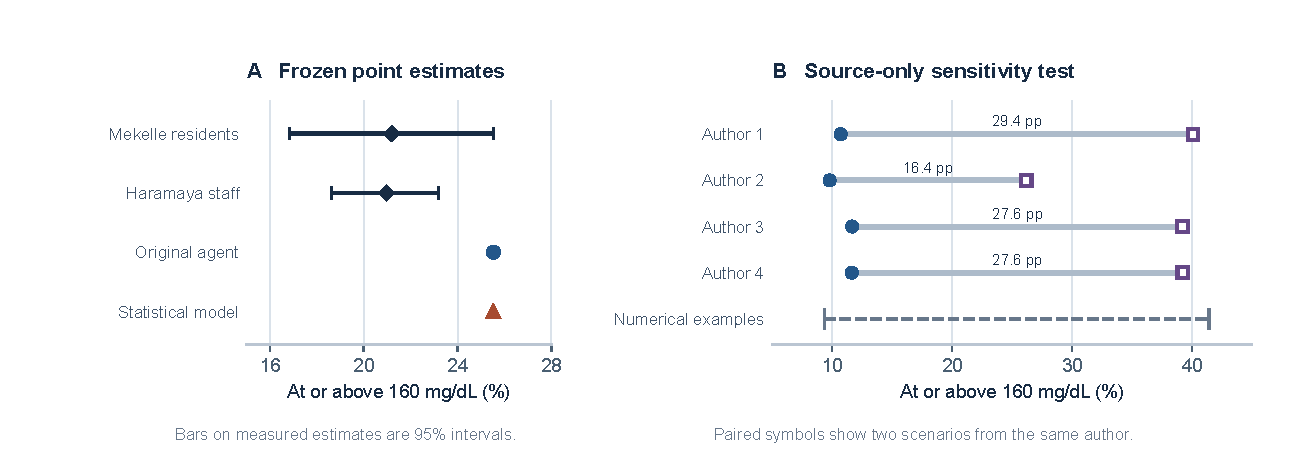
\includegraphics[width=.94\textwidth]{figures/nonhdl-selection.pdf}
\caption{What can a lipid screening study infer from the source? (A) A frozen agent and a statistical model independently selected similar joint laws. Diamonds and 95\% stratified bootstrap intervals summarize the two measured samples. (B) Four fresh authors received the same source summaries and were explicitly asked for two different, admissible joint models. Each line connects the pooled screening estimates for one author. The dashed segment joins two independently constructed numerical examples. The scenarios measure sensitivity at source.}
\Description{The original agent and comparator place about a quarter above the cutoff. In the separate experiment all four agents construct pairs of admissible models whose screening fractions differ by more than 16 percentage points.}
\label{fig:nonhdl}
\end{figure*}

\section{What a lipid paper leaves open about screening}
\label{sec:nonhdl}
For a researcher planning a screening study, mean non-HDL cholesterol and the number of people with an elevated value answer different questions. We fixed both analyses before reading either measured outcome. The two references were adult residents of Mekelle and permanent employees of Haramaya University, separately recruited in northern and eastern Ethiopia~\cite{mekelle,haramaya}. Both measured total cholesterol (TC) and HDL in fasting venous serum. We analyzed the complete paired records of participants aged 20 or older, including people taking medication. Our cutoff of 160 mg/dL defines the laboratory finding used for this comparison.

\paragraph{What was supplied?}
Both methods received the same published entries for 170 municipal adults in Mwanza, Tanzania~\cite{kavishe}. The source reports weighted means of 4.72 mmol/L for TC and 1.39 for HDL, hence 3.33 for non-HDL. It also gives the mean of individual TC/HDL ratios (3.66) and two single-marker threshold frequencies. We fitted common positive lognormal margins to the reported means and frequencies. The order statistics for both markers were identical across methods and sites. Any permutation therefore preserves the mean difference exactly. The proportion with TC minus HDL at least 160 still depends on which values are paired.

\paragraph{What did the agent choose?}
One fresh GPT session received the research request and source extract. It derived a Gaussian copula parameter from the published mean ratio and wrote a sampler that assigns HDL ranks conditionally on TC ranks. An independently specified statistical generator chose the same family and moment. The agent had no access to that implementation. They gave different individual assignments. Their mean ratios over three draws were 3.659 and 3.658, close to the reported 3.66. The raw interface rejected the field names in the agent's decision record. Before accessing either target, we registered a translation of metadata keys and executed the original code and scientific parameters in isolation. The comparison below concerns that execution.



\paragraph{Which use transferred?}
The common virtual mean was 128.77 mg/dL, compared with measured means of 125.12 in Mekelle and 123.58 in Haramaya. We did not assign a pass criterion to the mean. The primary threshold fraction was 25.53\% for the agent and 25.52\% for the statistical generator (Figure~\ref{fig:nonhdl}A). In Mekelle 68 of 321 participants reached the cutoff (21.18\%); in Haramaya 244 of 1,164 did (20.96\%). We had defined a study-planning tolerance of 20 additional people per 1,000. For the agent, the interval for the excess was $-0.02$ to 8.70 percentage points in Mekelle and 2.33 to 6.89 in Haramaya. The community result is unresolved under this rule. The employee result exceeds its upper limit. The statistical arm gave the same classifications. Both rates are sample estimates; the two recruitment frames afford separate checks within one country. The design compares transport of the complete laws. It cannot attribute the overestimate to pairing alone.

\paragraph{Can the agent construct the alternative?}

Four fresh GPT sessions each wrote a program for two pairings using only the same source packet and fixed marginal values. They knew the requested analysis and saw neither the Ethiopian estimates nor the numerical comparator. We sealed all programs before execution, used three fixed seeds per scenario, and independently recomputed the checks. All 24 tables retained the exact marginal arrays, placed HDL at or below TC for every virtual person, and reproduced the reported mean individual ratio to within 0.00020. The non-HDL mean stayed at 128.77. Each author's two screening rates differed by 16.37--29.35 percentage points (Figure~\ref{fig:nonhdl}B). One calibrated opposite rank cycles to the same ratio. The other three used swaps guided by the screening threshold. A numerical assignment procedure found admissible examples at 9.38\% and 41.41\%. Their spread shows why the original agreement at 25.5\% supplies little evidence about which estimate to use. These deliberately different model pairs establish feasibility. Their frequency in a patient population remains unknown (Appendix~\ref{app:pairingtest}).

In a separate prospective study, eight advisers ranked six uses before opening a Virginia community sample. All groups prioritized mean non-HDL, which fell outside its tolerance. Seeing the alternative pairings moved the screening use to last place. Appendix~\ref{app:virginia} reports every decision and measured outcome.

\paragraph{Using the model in another population.}
The virtual mean individual TC/HDL ratio of 3.659 met its prespecified margin in both later US survey periods. Updating two single-marker means increased screening error by 8.72 percentage points on the original pairing in both periods (Appendix~\ref{app:historicalmeans}).

\section{Source selection and measured agreement}
\label{app:ocular}
\paragraph{Returning to the corneal-thickness article.}
The author selected Hong et al.~\cite{hongpachymetry}, a study of 50 eyes from 30 healthy volunteers. In a subsequent development run it requested Table~3 and read its signed limits of agreement, $-14.9$ to $7.6~\mu$m. Their width yields an agreement-scale SD of $5.74~\mu$m under the article's correction for measurement error. The author retained an assumed ultrasound mean of $540~\mu$m and SD of $30~\mu$m. The generated means for Visante and ultrasound were 536.4 and $540.0~\mu$m. Table~1 reported 520.5 and $524.2~\mu$m. A shared offset cancels in their difference. Under a normal difference model, the model's return to the source changed the virtual absolute-discrepancy rate above $20~\mu$m from 0.22\% to 0.21\%. A $t_5$ difference model with the revised mean and variance gave 0.87\%. Six tables used three seeds per model, with 10,000 virtual eyes per table. The source did not provide a measured threshold count. This previously seen case documents a particular evidence decision.

\paragraph{Prospectively withholding eye-pressure measurements.}
The evaluator supplied Pye's article~\cite{pyeiop} with its table values and figure captions. The generative author had no access to the spreadsheet or plotted individual points. The research request specified the signed event, Pascal pressure minus Goldmann pressure greater than 3~mmHg in the same left eye. Means of the two instruments already determine the signed mean difference to printing precision. The author proposed a primary paired Gaussian law plus heavy-tailed and skewed alternatives. The primary estimate was 30.83--30.98\% across three seeds. The heavy-tailed law gave 28.37--28.42\%, closer to the observed 29/100, but produced nonpositive pressures and failed the prespecified absolute-tail check. The skewed alternative also failed that check. Hence no pair of eligible models met the sensitivity criterion. An independent reader recomputed the measured result and its bootstrap interval (20--38\%). The interval concerns sampling variation in the measured cohort. The range across seeds describes simulation variation. The paper also reported an absolute event at a different cutoff. The count for that diagnostic was 19/100 in the text and 21/100 in the workbook. Both counts were retained.

\paragraph{Selecting a BMI study and predicting a withheld tail.}
The selector chose Chia et al.~\cite{chiamalaysia} from two screened studies before the evaluator opened the same-study supplement. The prespecified population required adult complete pairs. Of 2,781 source rows, 13 lacked age and 10 were under 18, leaving 2,758. For each person the difference was self-reported minus measured BMI. The mean difference was $-0.0512$~kg/m$^2$ and 151 differences were strictly below $-2$~kg/m$^2$ (5.475\%, bootstrap 95\% interval 4.60--6.31\%). Six construction sessions were assigned. One exhausted its design output allowance and produced no model. All five completed primary models estimated a mean difference close to zero. Their seed medians for the threshold event ranged from 13.06\% to 17.06\%. Across the six assigned sessions, five met the $0.30$~kg/m$^2$ margin for the mean, zero met the three-percentage-point margin for the event, and zero met both. The prespecified single-case criterion required at least four sessions meeting both. The study produced 39 final tables and used 21 model calls. A secondary audit examined a published four-by-four table of BMI categories. All five authors explicitly left those cell counts unenforced. The paper reported 2,462/2,781 (88.53\%) in the same category for both measurements. The 15 primary virtual tables gave 72.22--76.51\%. The audit documents an available constraint and its consequence for category agreement. The effect of enforcing it on the continuous tail remains untested.


\end{document}
